%%%%%%%%%%%%%%%%%%%%
% CHAPTER 3
% %%%%%%%%%%%%%%%%%%

% This chapter's gonna be dense like the last one.\steezybreak\\
% We will begin with a discussion of unital and non-unital rings (\textit{rngs} lol) and we will look closely at a non-commutative ring whose elements commute with real numbers (Quaternions). We will discuss integral domains and then divisions rings which will naturally lead to more finite ring examples and then we will quickly introduce fields as commutative division rings. (don't worry we will include a venn diagram to simplify these differences between Groups, Rings, Integral Domains, and Commutative division rings (fields) ). Then we will discuss ring homomorphisms, Ideals, and Quotient Rings. Then we will look at Euclidean and Polynomial rings and we will build up some elementary results of Galois Theory. Then a bunch of Field/Ring thms will be staring us in the face and we will dive deeper with fields in Ch. 4 (setting the stage for a discussion of Modules and Vector Spaces).


\chapterimage{chapter_head_1.pdf} % Chapter heading image

\chapter{Ring Theory}
\vspace{-0.5in}
\section{Definition and Examples of Rings}
\href{https://en.wikipedia.org/wiki/David_Hilbert}{David Hilbert (1862-1943)} originally coined the term `Ring'. Hilbert was a German mathematician who had a profound impact on mathematics developed during the 19th and early 20th centuries\footnote{\href{https://en.wikipedia.org/wiki/Brouwer\%E2\%80\%93Hilbert_controversy}{Among other great mathematicians! We would be doing a disservice to the reader if we failed to mention that Hilbert could be a bit of a prickly fellow, effectively \textit{silencing} views from the constructivist "intuitionism" school of thought which opposed his "formalism".} The contributions of \href{https://en.wikipedia.org/wiki/L._E._J._Brouwer}{L. E. J. Brouwer} were also tremendous and perhaps more relevant to a reader interested in the modern foundations of mathematics. Throughout this book so far we have implicitly assumed the law of the excluded middle (typically in the form of "double negation elimination") as a viable tool in our arguments. Towards the end of the text, we will revisit some arguments and see where this concept crops up... for now, don't worry too much. Sorry for the diatribe just felt like it ought to go right next to my first mention of Hilbert lol.}. 

\begin{definition}[Ring]
A non-empty set $R$ is a \textit{ring} if in $R$ there are defined two binary operations denoted $\cdot$ and $+$ such that
\begin{enumerate}[label=\roman*)]
    \item $a,b \in R \implies a+b \in R$
    \item $a+b=b+a \ \forall \ a,b \in R$
    \item $(a+b)+c = a+(b+c) \ \ \forall \ a,b,c \in R$
    \item $\exists \ $an element "$0$" in $R \ \ni \ a+0=a \ \forall \ a \in R$
    \item $\forall \ a\in R \ \exists -a\in R \ni \ a+(-a)=0$
    \item $a,b\in R \ \implies a\cdot b \in R$
    \item $a\cdot (b\cdot c) = (a\cdot b)\cdot c \ \ \forall \ a,b,c \in R$
    \item $a\cdot (b+c) = (a\cdot b)+(a\cdot c)$ and $(b+c)\cdot a = (b\cdot a)+(c\cdot a) \ \ \forall \ a,b,c\in R$
\end{enumerate}
Note that (i)-(v) imply that $R$ is an abelian group under $+$. \steezybreak\\
If $R$ has an element called "$1$" with the property that 
\begin{align}
    a\cdot 1 = a = 1\cdot a \ \ \ \forall \ a\in R \nonumber
\end{align}
Then $R$ is \textit{a ring with unit element}. \steezybreak\\
If $a\cdot b=b\cdot a \ \ \forall \ a,b\in R$, then $R$ is \textit{a commutative ring}.
\end{definition}
\newpage
\begin{definition}[Complex Numbers] 
\begin{align}
    \mathbb{C} = \{a+bi \ |\ a,b\in \R\} \ \text{ with } i^2=-1 \nonumber
\end{align}
In $\mathbb{C}$, addition and multiplication are defined as follows:\steezybreak\\
Addition:
\begin{align}
    (a+bi)+(c+di) \underset{\text{add like terms}}{=} (a+c)+(b+d)i \nonumber
\end{align}
Multiplication:
\begin{align}
    (a+bi)(c+di)&=ac+bci+adi-bd \nonumber \\
    &= (ac-bd)+(bc+ad)i \nonumber
\end{align}
\end{definition}
Consider the following chain of inclusions 
\begin{align}
    &\mathbb{C} \ \ \ \ \ \leftarrow \ \R \ \ \leftarrow \mathbb{Q} \leftarrow \Z  \nonumber \\
    &\frac{n}{1}+0i \leftarrow \frac{n}{1} \leftarrow \frac{n}{1} \leftarrow n \nonumber
\end{align}
Each of the above are commutative rings with unit element under $\ \cdot$ and $+$ \steezybreak\\
Let's look at some other examples of rings aside from the integers, rationals, reals and complex numbers:
\begin{enumerate}\setcounter{enumi}{1}
    \item $2\Z=\{\text{ even integers }\}$ under usual $+$ and $\cdot$ \ \ \\
    \begin{align}
        \text{Note that } 2n(m)=2n  \ \text{ only when }m=1, \ \text{ but } 1\not\in 2\Z \nonumber
    \end{align}
    So $2\Z$ is a commutative ring without unit element. A ring without an unit element is often referred to as a \textit{rng}.
    \item $\Z_n=\{\underset{"0" + id}{0},\underset{"1" \cdot id}{1},2,\cdots,n-1\}$ under $\ +\mod n$ and $\cdot \mod n$ is a commutative ring with unit element (proof later).
    \item $M_2(\Z)$, $2\times 2$ matrices with integer entries
    \begin{align}
        ``0" \text{ is }\begin{bmatrix}0&0\\0&0\end{bmatrix} \nonumber \\
        ``1" \text{ is }\begin{bmatrix}1&0\\0&1\end{bmatrix} \nonumber 
    \end{align}
    Non-commutative since:
    \begin{equation*}
        \begin{drcases}
            \begin{bmatrix}
                    1&0\\1&0
            \end{bmatrix}
            \begin{bmatrix}
                    1&1\\0&0
            \end{bmatrix} &= \begin{bmatrix}
                    1&1\\1&1
            \end{bmatrix} \\
            \begin{bmatrix}
                    1&1\\0&0
            \end{bmatrix}\begin{bmatrix}
                    1&0\\1&0
            \end{bmatrix} &= \begin{bmatrix}
                    2&0\\0&0
            \end{bmatrix} 
        \end{drcases} \neq \ \therefore \text{ non-commutative}
    \end{equation*}
    Generalizing, $M_n(R)=\{n\times n \text{ matrices with ring entries}\}$ (where $R$ is a ring with unit element) is a non-commutative ring with ``$1$"
\end{enumerate}

\begin{figure}[h!]
    \centering
    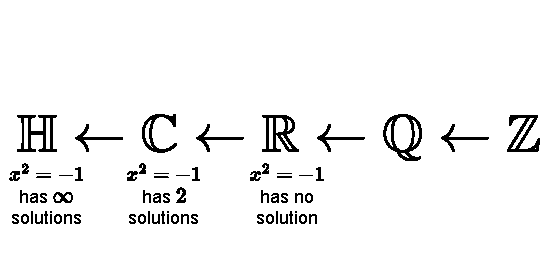
\includegraphics{Figures/Quaternions_xsquared_solns.pdf}
    \label{fig:x_squared_solns}
\end{figure}
\newpage
Let's have a look at another ring which generalizes the Complex numbers known as the Quaternions. The elements in this ring commute with real numbers but in general the ring is non-commutative. The Quaternions were first described by the Irish mathematician William Rowan Hamilton (1805-1865) in 1843. Hamilton had seen the utility of the commutative division ring $\C$ for describing points in a 2D plane which had the added benefit of "products" corresponding to rotations and re-scalings of points in the plane. Since points in 3 dimensional space can be described with triples $(x,y,z)$, Hamilton sought a convention for describing 3-D points in space in a manner similar to how the complex numbers describe 2-D points on a plane. On Monday 16 October 1843 in Dublin, whilst walking with his wife to a council meeting of the Royal Irish Academy, Hamilton made a revelation. In his excitement he carved a fundamental correspondence for what would be come known as the ``Quaternions" into the stone of Brougham bridge in Dublin. 
\begin{center}
    \begin{equation}
        i^2=j^2=k^2=ijk=-1 \nonumber
    \end{equation}
\end{center}
The next day in a letter to his friend and fellow mathematician John T. Graves, Hamilton summarized:
\begin{quote}
    And here there dawned on me the notion that we must admit, in some sense, a \textit{fourth} dimension of space for the purpose of calculating with triples ... An electric circuit seemed to close, and a spark flashed forth.
\end{quote}
Hamilton realized that in order to describe 3-D points in a ring whose products behave as rotations and re-scalings, he must admit an extra dimension. In fact, Ferdinand Georg Frobenius later proved in 1877 that for a division algebra over the real numbers to be finite-dimensional and associative, it \textit{cannot} be three-dimensional, and there are only three such division algebras: 
$\mathbb{R,C}$ (complex numbers) and $\mathbb{H}$ (quaternions) which have dimension 1, 2, and 4 respectively. Quaternions are typically denoted with the blackboard bold H ($\mathbb{H}$) in honor of Hamilton.
\begin{enumerate}\setcounter{enumi}{4}
    \item The Ring of Quaternions $\H$
\end{enumerate}
\begin{definition}[Quaternions $\H$]
\begin{align}
    \mathbb{H} &= \text{The ring of Quaternions} \nonumber \\
    &= \{a+bi+cj+dk \ | \ a,b,c,d \in \R \} \nonumber \\
    \text{ Where } &i^2=-1 \nonumber \\
    &j^2=-1 \nonumber \\
    &ji=-ij  \ \ \ \ (\leftarrow \text{ non-commutative})\nonumber \\
    &k=ij \nonumber \\
    &i,j,k \text{ commute with reals.}\nonumber
\end{align}
\end{definition}
Prove: $jk=i$
\begin{align}
    jk=jij&=-ijj \nonumber \\
    &= -i(-1) \nonumber \\
    &= i \nonumber
\end{align}
Prove $k^2=-1$:
\begin{align}
    k^2 = (ij)(ij) &= i(ji)j \nonumber \\
    &= i(-i)jj \nonumber \\
    &= -iijj \nonumber \\
    &= -(-1)(-1) \nonumber \\
    &= -1 \nonumber
\end{align}
\begin{figure}
    \centering
    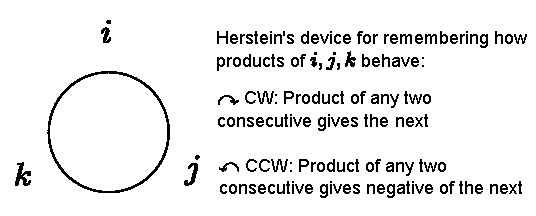
\includegraphics{Figures/Herstein_quat_device.pdf}
    \label{fig:herstein_quat_device}
\end{figure}
\subsection*{Example of how to Calculate products in $\mathbb{H}$}
\begin{align}
    + \ &: \ \text{ add "like" terms}\nonumber \\
    \circ \ &: \ \text{ distribute, use relations}\nonumber
\end{align}
\begin{align}
    & (i+2j+3k)(5i-j+k) \nonumber \\
    &=i(5i-j+k)+2j(5i=j+k)+3k(5i-j+k) \nonumber \\
    &= 5\underbrace{i^2}_{-1}-\underbrace{ij}_{k}+\underbrace{ik}_{-j}+10\underbrace{ji}_{-k}-2\underbrace{j^2}_{-1}+2\underbrace{jk}_{i}+15\underbrace{ki}_{j}-3\underbrace{kj}_{-i}+3\underbrace{k^2}_{-1} \nonumber \\
    &= -5-k-j-10k+2+2i+15j+3i-3 \nonumber \\
    &= -6+5i+14j-11k \nonumber
\end{align}

\noindent A quaternion $q=a+b\,\mathbf {i} +c\,\mathbf {j} +d\,\mathbf {k}$ , consists of a scalar part and a vector part. The quaternion $ b\,\mathbf {i} +c\,\mathbf {j} +d\,\mathbf {k} $ is called the vector part (sometimes imaginary part) of $q$, and $a$ is the scalar part (sometimes called the real part) of $q$. A quaternion that equals its real part (that is, its vector part is zero) is called a scalar or real quaternion. A quaternion that equals its vector part is called a vector quaternion. To avoid confusion we want to demonstrate a quick example which exemplifies some differences between dot product (inner product), cross product, and the product in $\mathbb{H}$.
\begin{align}
    \overrightarrow{v}&= i+2j+3k &\nonumber \\
    \overrightarrow{w}&= 5i-j+k &\nonumber \\
    \overrightarrow{v}\cdot \overrightarrow{w} &= (1)(5)+(2)(-1)+(3)(1)=5-2+3=6 \ \ \ \ \ \ \ \ \ &\text{(dot product)}\nonumber \\
    \overrightarrow{v}\times \overrightarrow{w} &= \det\left(\begin{bmatrix}
            i&j&k \\ 1&2&3 \\ 5&-1&1
    \end{bmatrix}\right) = 5i+14j-11k \ \ \ \ \ \ \ \ \ &\text{(cross product)}\nonumber \\
    (\overrightarrow{v}\times \overrightarrow{w})\times \overrightarrow{y} &\neq \overrightarrow{v}\times (\overrightarrow{w}\times \overrightarrow{y}) &\text{(cross products are non-associative)}\nonumber \\
    (\overrightarrow{v}\overrightarrow{w})\overrightarrow{y}&\underset{\cdot \text{ in } \mathbb{H} \text{ assoc.}}{=}\overrightarrow{v}(\overrightarrow{w}\overrightarrow{y}) \ \ \ \ \ \ \ \ \ &\text{(product in }\mathbb{H})\nonumber
\end{align}
\newpage
That being said, there is a relationship between the product used in $\mathbb{H}$ and the dot and cross products. If we adopt a convention of writing our quaternions as a scalar (real part) plus a vector (imaginary parts) $a=a_0+\overrightarrow{a}$ then we get:
\begin{align}
    ab &=(a_0+\overrightarrow{a})(b_0+\overrightarrow{b}) \nonumber \\
    &= (a_0b_0 - \overrightarrow{a}\cdot \overrightarrow{b}) + a_0 \overrightarrow{b}+b_0\overrightarrow{a}+\overrightarrow{a}\times \overrightarrow{b} \nonumber 
    \end{align} (See footnote regarding line above\footnote{Try demonstrating this correspondence yourself! To help perhaps first try to demonstrate this: \\ $(a_0+a_1i+a_2j+a_3k)(b_0+b_1i+b_2j+b_3k)= (a_0b_0-a_1b_1-a_2b_2-a_3b_3)+(a_0b_1+a_1b_0+a_2b_3-a_3b_2)i+(a_0b_2+a_2b_0+a_3b_1-a_1b_3)j+(a_0b_3+a_3b_0+a_1b_2-a_2b_1)k$ This can be accomplished by distributing, simplifying products between $i,j,k$ using Herstein's device, and collecting the scalar, $i$, $j$, and $k$ terms, respectively.})
    \begin{align}
    &\implies \frac{1}{2}(ab-ba)=\overrightarrow{a}\times\overrightarrow{b} \nonumber
\end{align}
the last implication comes from anticommutativity of cross product (i.e. $\overrightarrow{a}\times \overrightarrow{b}= (-\overrightarrow{b}\times \overrightarrow{a})$) and commutativity of dot product. 

You may recall from earlier encounters with vectors that vector cross products only exist in 3 and 7 dimensions. One may ask, why only 3 and 7? Without going off on too much of a tangent I will leave this for interested readers to research in their own time: The nonexistence of nontrivial vector-valued cross products of two vectors in other dimensions is related to Hurwitz's theorem (composition Algebras) that implies the only normed division algebras are ones with dimension 1, 2, 4, and 8, these correspond to the reals, complex numbers, quaternions, and octonions, respectively.
\begin{tcolorbox}
\begin{center}
    From now on, we will assume ring $R$ is a ring with unit element, i.e. we will assume $R$ has ``$1$", multiplicative identity
\end{center}
\end{tcolorbox}
\section{Basic Ring Properties}
\begin{lemma}[Basic Ring Properties]
If $R$ is a ring, then $\forall a,b\in R$
\begin{enumerate}[label=(\roman*)]
    \item $a0=0a=0$
    \item $a(-b)=(-a)b=-(ab)$
    \item $(-a)(-b)=ab$
    \item $(-1)a=-a$
    \item $(-1)(-1)=1$
\end{enumerate}
\noindent\textit{Proof:}
\begin{enumerate}[label=(\roman*)] 
\item We will show $a0=0$ first, and leave $0a=0$ to the readers (use an \textit{almost} identical argument)
\begin{align}
        a0&=a(0+\underbrace{0}_{+ id.})=a0+a0 \nonumber \\
        a0&\in R \ \ \ \ \ (\ \cdot \text{ closure }) \nonumber \\
        R \text{ abelian group under }+ &\implies -(a0)\in R \nonumber
    \end{align}
    Now adding $-(a0)$ to both sides:
    \begin{align}
        \underbrace{a0+[-(a0)]}_{0 \text{ inv. prop.}}&=a0+\underbrace{[a0+[-(a0)]]}_{0 \text{ inv. prop.}} \nonumber \\
        0&=a0+0 \nonumber \\
        0&= a0 \nonumber
    \end{align}
    Note that $0a=0$ follows the same method of proof but we use right side distribution.
    \item Here we will first show $a(-b)$ is the additive inverse of $ab$ which will imply that $a(-b)$ is $-(ab)$:
    \begin{align}
        a(-b)+ab&= a[(-b)+b] \ \ \ \ \ &(\text{ l-distribution}) \nonumber \\
        &= a[0] \ \ \ \ \ &(\text{ property of additive inverses}) \nonumber \\
        &= 0 \ \ \ \ \ &(\text{ previous prop }) \nonumber \\
        &= ab+a(-b) \ \ \ \ \ &(R \text{ abelian under +}) \nonumber
    \end{align}
    By uniqueness of additive inverses, $a(-b)$ is additive inverse of $ab$. \\ $\therefore \ \  a(-b)=-(ab)$. \\ For the other one (i.e. in order to show $(-a)b=-(ab)$  ) we need the other distributive law.
    \item We wish to show $(-a)(-b)=ab$ to do so we will use the property we just proved in (ii) now thinking of $-a$ as $a$ and using a property of inverses in groups we uncovered in Chapter 2.
    \begin{align}
        (-a)(-b)&= -[(-a)b] \ \ \ \ \ & (-a \text{ is a ring elt. use (ii) w/ }-a \text{ as }a ) \nonumber \\
        &= -[-(\underbrace{ab}_{\in R \ (\ \cdot \text{ closure})})] \ \ \ \ \ & ( \text{property (ii) again}) \nonumber \\
        &= (ab) \ \ \ \ \ & (\ R\text{ is a group under }+: (g^{-1})^{-1}=g) \nonumber
    \end{align}
    \item \begin{align}
        (-1)a&= -(1\cdot a) \ \ \ \ \ & ( \text{property (ii)}) \nonumber \\
        &= -(a) \ \ \ \ \ & (\text{mult. identity}) \nonumber \\
        &= -a \nonumber
    \end{align}
    \item \begin{align}
        (-1)(-1)&= (1)(1)  \ \ \ \ \ & (\text{property (iii) with }a=b=1) \nonumber \\
        &= 1 \nonumber
    \end{align}
    $\blacksquare$
\end{enumerate}
\end{lemma}

\begin{definition}[Zero Divisors]
If $R$ is a commutative ring, $a,b\in R$ are \textit{zero divisors} if $a\neq 0$ and $b\neq 0$ but $ab=0$.
\end{definition}
\begin{definition}[Integral Domain]
A commutative ring $R$ (with unit elt) is an \textit{integral domain} if it has no zero divisors. (i.e. if $ab=0$, either $a=0$ or $b=0$)
\end{definition}
\subsection*{Examples}
\begin{example}
$\Z,\Q,\R,\C$ are integral domains.
\end{example}
\begin{example}
$\Z_{10}=\{0,1,2,3,4,5,6,7,8,9\}$ under $+\mod 10$ and $\cdot \mod 10$ is not an integral domain...
\begin{align}
    5\cdot 2 &= 10\mod 10 = 0 \nonumber \\
    &\therefore \ 5,2 \text{ are zero-divisors} \nonumber
\end{align}
\end{example}

\begin{example}
$M_2(\Z)$ is not an integral domain because it is not a \textul{commutative} ring.
\begin{align}
    AB= \begin{bmatrix}
            0&0\\0&0
    \end{bmatrix} = 0 \ \ \ \text{ for } A= \begin{bmatrix}
            1&0\\1&0
    \end{bmatrix}, \ \ \ B= \begin{bmatrix}
            0&0\\1&1
    \end{bmatrix}, \ \ \ \ BA = \begin{bmatrix}
            0&0\\2&0
    \end{bmatrix} \nonumber
\end{align}
$A$ and $B$ are zero-divisors
\end{example}
\newpage

\begin{example}[Example from Pg 130 \#10 in Herstein Text] \hspace{0.1in }\\
A commutative ring $R$ is an integral domain $\iff$ $\forall \ a,b,c \in R$ with $a\neq 0$, $ab=ac \implies b=c$

\textit{Proof:} \steezybreak\\
$\Rightarrow$: Assume $R$ is an integral domain; so $R$ has no zero divisors. Now suppose $ab=ac$ with $a\neq 0$.
\begin{align}
    ac\in R &\implies \exists \ -(ac)\in R & (R +\text{ group}) \nonumber \\
    ab+[-(ac)]&= ac + [-(ac)] & \nonumber \\
    ab+a(-c)&=0 & ( \text{ (ii) }) \nonumber \\
    a[b+(-c)]&=0 & (\text{ Dist. Law}) \nonumber
\end{align}
Since $R$ has no zero divisors, and $a\neq 0$ 
\begin{align}
    &\implies b+(-c)=0 \nonumber \\
    &\implies b+(-c)+c= c \nonumber \\
    &\implies b+0= c \nonumber \\
    &\implies b=c \nonumber
\end{align}
$\Leftarrow$: For this direction we assume cancellation property holds and we will show $R$ has no zero divisors. Suppose $ab=0$ with $a\neq 0$ we'll show $b$ is forced to be $0$.
\begin{align}
    ab&=0 & \nonumber \\
    &= a0 &(\text{ Lemma 3.2.1 part (i) }) \nonumber
\end{align}
Cancellation of $a$ gives
\begin{align}
    b=0. \ \ \ \ \blacksquare \nonumber
\end{align}
\end{example}
Quick takeaways, given $R$ commutative ring,
\begin{align}
    R \text{ is an integral domain} &\iff R \text{ has no zero divisors} \nonumber \\
    &\iff R \text{ has cancellation property.} \nonumber
\end{align}

\begin{definition}[Division Ring]
    A ring $R$ with unit element is a \textit{division ring} if its non-zero elements form a group under ``$\cdot$" (i.e. if $R$ has the additional property of multiplicative inverses for all $a\neq 0 \in R$). \steezybreak\\
    
    \noindent Even more compact: $R \text{ div. ring} \iff \forall a \in R \ni a\neq 0, \exists b \in R \ni ab=1$.
\end{definition}

\begin{example}
    $\Z$ is \textul{not} a division ring since $2b=1$ is never true for $b\in \Z$ ($2$'s multiplicative inverse is $\frac{1}{2} \not \in \Z$)
\end{example}
\begin{example}
    $\Q$ is a division ring, so are $\R$, and $\C$. In fact they are all commutative division rings: \steezybreak\\
    
    \begin{align}
        \text{Let }  a/b \in \Q \text{ with } a,b\neq 0,  \ &\implies (\frac{a}{b})^{-1} = \frac{b}{a} \nonumber \\
        r \in \R, r\neq 0 &\implies r^{-1}=\frac{1}{r} \nonumber \\
        (a+bi)\in \C \text{ with $a,b$ not BOTH zero} &\implies (a+bi)^{-1} = \frac{a}{a^2+b^2} - \frac{b}{a^2+b^2}i \nonumber
    \end{align}
    Left to the reader to confirm that $(a+bi)^{-1}$, as given, satisfies $(a+bi)(a+bi)^{-1} = 1+0i$
\end{example}

\begin{example}
    $\H$ is a non-commutative division ring
    \begin{align}
        \H = \{a+bi+cj+dk \ | \ a,b,c,d \in \R \} \text{ with } i^2=j^2=k^2=-1, ji = -ij \nonumber
    \end{align}
    Recall Herstein's device for products of $i$ $j$ and $k$: 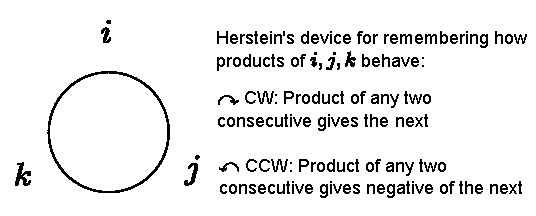
\includegraphics[width= 0.4\textwidth]{Figures/Herstein_quat_device.pdf} \steezybreak\\
    \noindent If $a+bi+cj+dk \in \H$ with $a,b,c,d$ not all zero we can denote $s= a^2+b^2+c^2+d^2$, then
    \begin{align}
        (a+bi+cj+dk)^{-1}&= \frac{a}{s} - \frac{b}{s}i - \frac{c}{s}j - \frac{d}{s}k\nonumber
    \end{align}
    A good exercise for the reader would be to prove by checking that the product $=1$ for left and right multiplication.
\end{example}

\begin{example} 
    $M_2(R)$ (where $R$ a ring) is a non-commutative ring but not a division ring:
    \begin{align}
        \det\begin{pmatrix}
            0&0\\1&1
        \end{pmatrix} = 0 \ \ \therefore \text{ has no inverse} \nonumber
    \end{align}
\end{example}

\begin{example}
    $GL_2(R)$ is not even a ring so not a division ring. $GL_2(R)$ does not have ``$e$" (identity) for ``$+$" operation.
\end{example}

\begin{definition}[Field] 
A \textit{field} is a commutative division ring.
\end{definition}

\subsubsection*{Exercise \#12 from Pg. 130 in Herstein:}
Prove every field is an integral domain.
\textit{Proof:} Say $F$ is a field, we'll show that $F$ has no zero divisors: \steezybreak\\
Suppose $ab=0$ and further assume $a\neq 0$ we must show this setup forces $b=0$
\begin{align}
    a\neq 0 &\implies \exists \ a^{-1}\in F \ \ (F\text{ is a div. ring}) \nonumber \\
    &ab=0 \nonumber \\
    &\implies a^{-1}ab =a^{-1}0 \nonumber \\
    &\implies 1b = a^{-1}0 \nonumber \\
    &\implies b=0 \nonumber
\end{align}
So $F$ has no zero divisors. $\blacksquare$ \steezybreak\\

A natural question one might ask, `` are there any finite fields?" will be answered shortly. Recall in $\Z_{10}$ we have that $5\cdot 2 = 0$, $\Z_{10}$ is certainly a ring, but it is not an integral domain and hence is not a field. How about $\Z_{7}$? In fact it is! but we will need to prove two more results to make it very clear, first we will prove ring $\Z_p$, has no zero divisors for $p$ prime (making it a finite integral domain). Then in the lemma that follows we will prove that a finite integral domain is a field.

\begin{proposition}[$p$ prime $\implies \Z_p$ integral domain] 
$\Z_p$ has no zero divisors for $p$ prime. \steezybreak\\
\textit{Proof:} Suppose $ab=0$ for $a,b \in \Z_p \ni \ a\neq 0$, we will show $b$ is forced to be zero. 

\noindent In $\Z$, $ab=0$ means $ab\equiv 0 \mod p$, i.e. $p|ab$. Now, $a\not\equiv 0 \mod p$ means $p\not | a$ so $p$ must divide $b$. Lastly $p|b \implies b\equiv 0 \mod p$
\begin{align}
    \therefore b=0 \text{ in } \Z_p \nonumber
\end{align}
So $\Z_p$ is a finite integral domain. $\blacksquare$
\end{proposition}

\begin{lemma}[Finite Integral Domain $\implies$ Field] 
A finite integral domain is a field. \steezybreak\\
\noindent \textit{Proof:}
To begin, we note that $R$ finite integral domain $\implies$ $R$ is a commutative ring with ``$1$" in which cancellation holds, and it is finite $R=\{x_1,x_2,\cdots, x_n\}$ $n-$distinct. Let $a\in R$ with $a\neq 0$, we must show that $a^{-1}$ exists in $R$. Consider the list:
\begin{align}
    x_1a, \ x_2a, \ x_3a, \cdots, \ x_na \ \ \ \text{ all }\in R \text{ by closure.} \nonumber
\end{align}
Are there duplicates? \\ 
Well if $x_ia=x_ja$, cancellation in $R$ $\implies \ x_i=x_j$ , \ \ $\Rightarrow\Leftarrow$. \\ 
So no, no duplicates exist in this list. The new list is just $R$ again. \\ 
Since $1\in R$ $\implies \ x_ia=1$ for some $1\leq i \leq n$, \\ 
$\therefore x_i$ is the required $a^{-1}$. $\blacksquare$
\end{lemma}
\begin{figure}
    \centering
    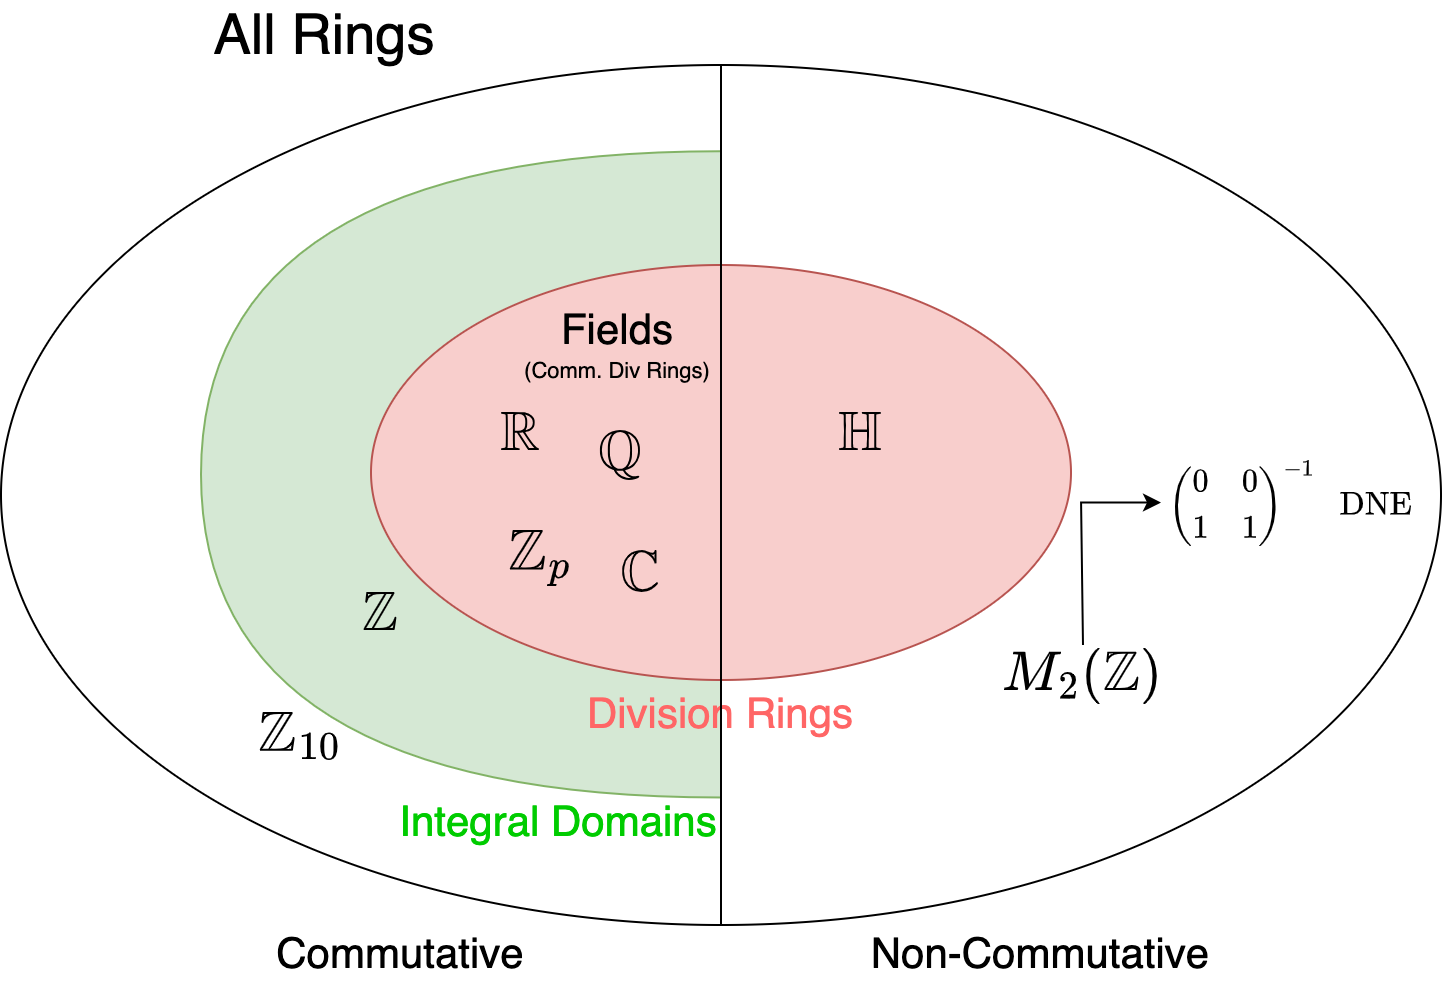
\includegraphics[width=0.9\textwidth]{Figures/Ring Classifications.png}
    \caption{Ring Classifications}
    \label{fig:ring-classifications}
\end{figure}
\subsection*{Characteristic of Integral Domains}
Suppose $R$ is an integral domain (w/ ``$1$"). Think of $R$ as an additive group and consider $o(1)$ (order of $1$):
\begin{align}
    o(1)=m = \text{ smallest positive integer }\ni \underbrace{1^m}_{\underbrace{1+1+\cdots+1}_{m \text{ times}}\ =} = \underbrace{0}_{\underbrace{0}_{``e" \text{ in additive }R}} \nonumber
\end{align}
\begin{definition}[Characteristic of Integral Domain]
\begin{enumerate}
    \item Integral domain $R$ has characteristic $0$, denoted $\characterisic(R)=0$, if the only $m\in \Z$ satisfying $1^m=0$ is $m=0$.
    \item If $\characterisic(R)\neq 0$, then $\characterisic(R)=o(1)$
\end{enumerate}
\end{definition}

\begin{example}
    $\Z$, $\R$, $\Q$, and $\C$ all have $\characterisic(R)=0$
\end{example}
\newpage
\begin{example}
    $\Z_p$, $p$ prime, has $\characterisic(R)=p$ \ \ \ \ \ ($\underbrace{1+1+\cdots +1}_{p \text{ times}} = 0$)
\end{example}
\noindent The Characteristic of an Integral Domain R is $o(1)=$ the order of the multiplicative identity in the additive group $R$.
\begin{align}
    \text{if }o(1)&=\infty \ \text{ then }\characterisic(R)=0 \nonumber \\
    \text{if }o(1)&=m\in \Z^{+} \ \text{ then }\characterisic(R)=m \nonumber
\end{align}
The characteristic affects the calculations in $R$: \\ 
Take $x,y\in R$
\begin{align}
    \text{Say }R \text{ has }\characterisic(R)=0, \text{ then} \nonumber \\
    (x+y)^2 &= (x+y)(x+y) \nonumber \\
    &= x^2+xy+yx+y^2 \nonumber \\
    &= x^2 + 2xy + y^2  \ \ \ (R\text{ comm.}) \nonumber 
\end{align}
Above we use additive notation $g+g=2g$ after recognizing that $R$ int. domain implies $R$ commutative.
\begin{align}
    \text{Say }R \text{ has }\characterisic(R)=2, \text{ then} \nonumber \\
    (x+y)^2 &= x^2 + 2xy + y^2  \nonumber \\
    &= x^2+\underbrace{(1+1)}_{\substack{o(1)=2 \\ \text{ so this is }0, \\ 0\cdot r = 0 \ (L3.2.1)}}xy+y^2 \nonumber \\
    &= x^2+y^2 \nonumber
\end{align}

\begin{definition}[Subring]
A subset $S$ of ring $R$ is a subring if
\begin{enumerate}[label=\roman*)]
    \item $S<R$ (under $+$).
    \item $1_R\in S$.
    \item $S$ is closed under $\cdot$ in $R$.
\end{enumerate}
$S$ inherits the rest of $R$'s ring properties:
\begin{itemize}
    \item $+$ abelian
    \item $\cdot$ associativity
    \item 2 distributive laws
\end{itemize}
$R$ is a ``trivial" subring of itself.
\end{definition}
\newpage
\begin{example}[Personal Ring Example] 
Discuss the ring generated by $A= \begin{pmatrix}
    0&0\\0&1
\end{pmatrix} \in M_2(\Z_2)$
    \begin{table}[h!]
    \centering
    \begin{tabular}{c||c|c|c|c|}
         $+$& $0$&$I$&$A$&$A+I$  \\ \hline \hline
         $0$&$0$&$I$&$A$&$A+I$\\ \hline
         $I$&$I$&$0$&$A+I$&$A$ \\ \hline
         $A$&$A$&$A+I$&$0$&$I$ \\ \hline
         $A+I$&$A+I$&$A$&$I$&$0$ \\ \hline
    \end{tabular} \hspace{0.2in}
    \begin{tabular}{c||c|c|c|c|}
         $\cdot$& $0$&$I$&$A$&$A+I$  \\ \hline \hline
         $0$&$0$&$0$&$0$&$0$\\ \hline
         $I$&$0$&\cellcolor{blue!25}$I$&\cellcolor{blue!25}$A$&\cellcolor{blue!25}$A+I$ \\ \hline
         $A$&$0$&\cellcolor{blue!25}$A$&\cellcolor{blue!25}$A$&\cellcolor{blue!25}$0$ \\ \hline
         $A+I$&$0$&\cellcolor{blue!25}$A+I$&\cellcolor{blue!25}$0$&\cellcolor{blue!25}$A+I$ \\ \hline
    \end{tabular}
    \caption{Cayley Table (additive) and Table of Products for ring generated by $A$. Note that $0$'s appearing in the sub-block shaded in blue $\implies$ 0 divisions $\implies$ $R$ is not an integral domain.}
    \label{tab:Cayley_and_products_ex_ring}
\end{table}\\
Relations:
\begin{align}
    2I&=0 \nonumber \\
    2A&=0 \nonumber
\end{align}
Ring of order 4. Symmetry down main diagonal of $\cdot$ table $\implies$ commutative. As we noted from the multiplication table ($\cdot$ table) $(A+I)A=0$ so we have zero divisors, $\therefore$ $R$ is not an integral domain. $R$ is a basic commutative ring.\\
\begin{figure}[h!]
    \centering
    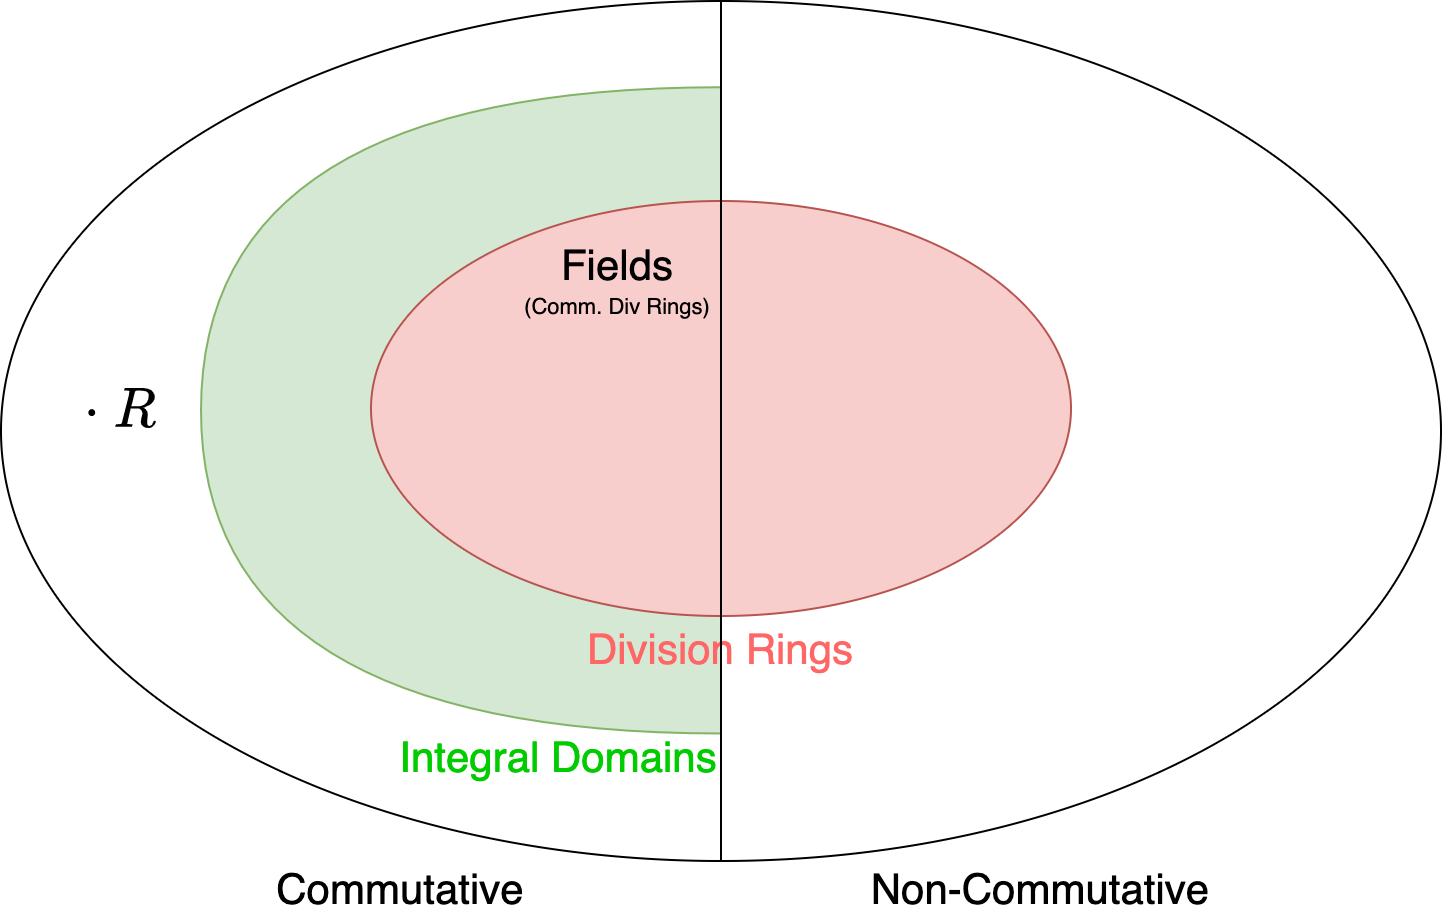
\includegraphics[width=0.65\textwidth]{Figures/Example_Ring_Figure.png}
    \caption{Where $R$ sits in our previous diagram}
    \label{fig:R_comm_ring}
\end{figure}\\
Let's explore the subrings of $R$ and see if there are any non-trivial ones. Looking back at part (i) of our definition of a subring we can begin by looking at $R$'s subgroups under addition:
\begin{center}
    \begin{tabular}{|l|c|} \hline
         \textbf{Order } & \textbf{Subgroup}  \\ \hline
         $4$ & $R$ \\ \hline
         $2$ & $\{I,0\}=\langle I \rangle, \{A,0\}=\langle A \rangle, \{A+I,0\}= \langle A+I \rangle$ \\ \hline
         $1$ & $\langle 0 \rangle $ \\ \hline
\end{tabular}
\end{center}
Now the next requirement for being a subring is that the subgroup needs to contain ``1", the multiplicative identity. So $\{A+I,0\}$ and $\{A,0\}$ are out of the running, but $\{I,0\}=\langle I \rangle$ is still a contender! Lastly we require the subgroup to be closed under $\cdot$, which $\{I,0\}$ is so $\{I,0\}$ is a subring!!

As an extra takeaway from this discussion, we can also see from that table of subgroups that $R$ must be non-cyclic since there is no single element of order $4$.
\end{example}
\newpage
\section{Ring Homomorphisms}
We've seen structure-preserving maps for groups (group homomorphisms), now we will extend the idea to Rings.
\begin{definition}[Ring Homomorphism] 
Let $R$, $R'$ rings. A map $\phi : R \rightarrow R'$ is a \textit{(ring) homomorphism} if $\forall \ a,b \in R$
\begin{enumerate}
    \item $\phi(a+b)=\phi(a)+\phi(b)$ 
    \item $\phi(a\cdot b) = \phi(a)\cdot \phi(b)$
\end{enumerate}
\end{definition}

\begin{lemma} 
If $\phi : R\rightarrow R'$ is a ring homomorphism, then
\begin{enumerate}
    \item $\phi(0)=0'$
    \item $\phi(-a)=-\phi(a)$
\end{enumerate}
\textit{Proof:}\\
We begin by first noting that $R$ and $R'$ are groups under $+$ (below we use the handles $G$ and $G'$ when thinking of $R$ and $R'$ simply as groups under their respective ``+" operations) and $\phi$ is a group homomorphism $\phi:G \rightarrow G'$. Then by Lemma 2.7.2 we have
\begin{align}
    \phi(e)&=e' \nonumber \\
    \phi(a^{-1}) &= \phi(a)^{-1} \ \forall \ a \in G. \ \ \ \blacksquare \nonumber
\end{align}
\end{lemma}

\begin{definition}[Kernel of Ring Homomorphism] 
Given $\phi:R\rightarrow R'$ ring hom. The \textit{kernel of} $\phi$ is defined:
\begin{align}
    \ker \phi = \{ a \in R \ | \ \phi(a)=0'\} \nonumber
\end{align}
\end{definition}

\begin{lemma}
Given $\phi: R \rightarrow R'$ ring homomorphism, then
\begin{enumerate}[label=\roman*)]
    \item $\ker \phi < R$ under $+$
    \item $\forall \ a \in \ker \phi $ and $\forall r \in R$, $ar, ra \in \ker\phi$
\end{enumerate}
\textit{Proof:}\\
\begin{enumerate}[label=\roman*)]
    \item Recall that Lemma 2.7.3 states that for group homomorphism $\sigma : G \rightarrow G'$ the kernel of $\sigma$ is a normal subgroup of $G$ (i.e. $\ker{\sigma} \ \triangleleft \ G$). Now, since $R$ and $R'$ are groups under $+$ and $\phi$ is a group homomorphism, $\ker{\phi} \ \triangleleft \ R$
    \item Take $a \ \in \ \ker{\phi} $ and $r \ \in \ R$
    \begin{align}
        \phi(ar) &= \phi(a)\phi(r) = 0' \cdot \phi(r)=0' \implies ar \ \in \ker{\phi} \nonumber
    \end{align}
    A similar argument can be made to show $\phi(ra)=0'$
\end{enumerate}

\end{lemma}

\begin{definition}[Ring Isomorphism]
    $R$ is isomorphic to $R'$ ($R\approx R'$) if $\exists$ a ring homomorphism $\phi : R \rightarrow R'$ that is bijective. Then $\phi$ is an \textit{isomorphism} (\textit{ring isomorphism})
\end{definition}

\begin{lemma}
    The ring hom. $\phi : R \rightarrow R'$ is injective $\iff$ $\ker\phi = \{0\}$ \steezybreak\\
    \textit{Proof:} Apply group theory. $\blacksquare$
\end{lemma}
\subsection*{Examples of Ring Homomorphisms}
\begin{example}
    The ``trivial map" $\phi: R \rightarrow R'$ where $\phi(a)=0'$ $\forall \ a \in R$
    \begin{align}
        \text{Take }a,b \ & \in R \nonumber \\
        \phi(a+b)&= 0' \nonumber \\
        &= 0' + 0' \nonumber \\
        &= \phi(a) + \phi(b) \nonumber
    \end{align}
    \begin{align}
        \phi(ab)&= 0' \nonumber \\
        &= 0'\cdot 0' \ \ \ \ \ \ \ \ \ \ \ \ (Lemma \ 3.2.1 \ (i)) \nonumber \\
        &= \phi(a)\cdot \phi(b) \nonumber
    \end{align}
    $\ker\phi = R$
\end{example}

\begin{example}
    The identity map: $\phi : R \rightarrow R$ where $\phi(r)=r$ $\forall \ r \in R$ \steezybreak\\
    $\ker\phi = \{0\}$
\end{example}

\begin{example}
Consider the following: $\phi: \Z \rightarrow \Q$ where $\phi(n) = \frac{n}{1}$ $\forall \ n \in \Z$. Is this a ring homomorphism? Is it injective? Surjective?

Take $m,n \in \Z$
\begin{align}
    \phi(m+n) &= \frac{m+n}{1} = \frac{m}{1}+\frac{n}{1}= \phi(m)+\phi(n) \nonumber
\end{align}
\begin{align}
    \phi(mn) &= \frac{mn}{1} = \frac{m}{1}\cdot\frac{n}{1}= \phi(m)\phi(n) \nonumber
\end{align}
So it is a ring homomorphism. Furthermore
\begin{align}
    \ker \phi &= \{n\in\Z \ | \ \frac{n}{1}=0\} = \{0\} \nonumber
\end{align}
so it is injective. $\phi$ is not surjective because $\frac{2}{3}$ (among many others) has no pre-image under $\phi$. $\phi$ is an embedding of $\Z$ into $\Q$ (change of perspective)
\end{example}

\begin{example}
Complex conjugation: define $\phi : \C \rightarrow \C $ by $\phi(a+bi)=a-bi= \underset{\substack{MINUS \\ notation \ meaning}}{\underbrace{a+(-b)i}}$ \steezybreak\\
Consider $a+bi, c+di \in \C$
\begin{align}
    \phi((a+bi)+(c+di))= \phi((a+c)+(b+d)i)&= (a+c)-(b+d)i \nonumber \\
    &= (a+c)+(-1)(b+d)i \nonumber \\
    &= (a+c)+[(-b)+(-d)]i \nonumber \\
    &= a+c +(-b)i+(-d)i \nonumber \\
    &= a-bi + c-di \nonumber \\
    &= \phi(a+bi)+\phi(b+di) \nonumber
\end{align}
\begin{align}
    \phi[(a+bi)(c+di)]&=\phi[(ac-bd)+(ad+bc)i] \nonumber \\
    &= ac-bd-(ad+bc)i \nonumber \\
    &= ac-bd-adi-bci \nonumber \\
    &= ac-adi -bci-bd \nonumber \\
    &= a(c-di)-bi(c-di) \nonumber \\
    &= (a-bi)(c-di) \nonumber \\
    &=\phi(a+bi)\phi(c+di) \nonumber 
\end{align}

\begin{align}
    \ker\phi = \{a+bi | \phi(a+bi)=0+0i\} = \{0+0i\} \nonumber
\end{align}
so $\phi$ is injective. \steezybreak\\ Furthermore, note that arbitrary complex number $r+si$ has pre-image $r-si$, 
\begin{align}
    \phi(r-si)=r-(-s)i=r+si \nonumber
\end{align}
so $\phi$ is surjective.
\end{example}
\section{Ideals and Quotient Rings}

\begin{definition}[Ideal (Two-sided Ideal)]
    A non-empty $U$ of ring $R$ is \textit{ideal} if 
    \begin{enumerate}[label=\roman*)]
        \item $U<R$ under $+$
        \item $\forall \ u \in U$ and $r \in R$, $ur\in U$ and $ru\in U$
    \end{enumerate}
    This second property is known as the absorption, or ``ideal" property.
\end{definition}
Let's look at subgroups from our previous example and see if they absorb...
\begin{align}
    \{0,I\}& \text{ is not ideal, }IA\not\in \{0,I\} \nonumber \\
    \{0,A\}& \text{ is and ideal, absorbs} \nonumber \\
    \{0,A+I\}& \text{ is  ideal } \nonumber \\
    \{0\}& \text{ is ideal} \nonumber
\end{align}

\subsection*{Examples of Ideals}
\begin{example}
    Every ring $R$ has two trivial Ideals: $\{0\}$ and $R$, both are subgroups under $+$, 
    \begin{align}
        r\cdot 0 = 0 = 0\cdot r \nonumber
    \end{align}
    so $\{0\}$ absorbs. $R$ absorbs by $\cdot$ closure.
    \begin{align}
        \underset{\in R}{r}\cdot \underset{\in R}{a} \in R\nonumber
    \end{align}
\end{example}

\begin{example}
    $\phi : R \rightarrow R'$ ring hom. then $\ker \phi$ is an ideal of $R$ (Lemma 3.3.2)
\end{example}

\begin{example}
    Let $R=\Z$, choose $n \in \Z$ and consider $n\Z = U = \{\cdots, -2n, -n, 0,n, \cdots\}$, is this an ideal of $R$? Lets begin by trying to show $U$ is a subgroup under $+$. Then we will show it has the ideal property
    \begin{enumerate}[label=\roman*)]
        \item \textbf{Subgroup under $+$} \\ Lemma 2.4.1 applies here since $n\Z \neq \emptyset$ (it contains 0)
        \begin{itemize}
            \item \textbf{+ Closure:} $\forall \ a,b\in \Z$
            \begin{align}
                \underset{\in n\Z}{an}+\underset{\in n\Z}{bn} = (a+b)n \in n\Z \nonumber
            \end{align}
            \item \textbf{+ Inverses:} $\forall \ a\in \Z$
            \begin{align}
                -(an) \underset{\substack{L\ 3.2.1\\pt.\ 2}}{=} \underset{\in \Z }{(-a)}n \in n \Z \nonumber
            \end{align}
        \end{itemize}
        \item \textbf{Ideal (Absorption) Property} \\ $\forall m \in \Z$, $\forall \ an \in n\Z$ we have:
        \begin{align}
            m(an)&=\underset{\in \Z}{(ma)}n \in n \Z \nonumber \\
            (an)m&=m(an) \in n \Z \ \ \ \ \ \ \ (\Z \text{ comm. under }\cdot)\nonumber
        \end{align}
    \end{enumerate}
    
    $\therefore \ $  $n\Z$ is an ideal in $\Z$.\\
     I'm going to box the findings of this example because it might come in handy down the road:
     \begin{tcolorbox}[width=2in, center=true]
\begin{center}
    $\forall \ n \in \Z$, $n\Z$ is an ideal in $\Z$.
\end{center}
\end{tcolorbox}
\end{example}

\begin{example}
Let $R=M_2(\Z)$ and $U=M_2(2\Z)$ \\
We will begin by showing $U<R$ under $+$
\begin{enumerate}[label=\roman*)]
    \item $U$ \textbf{nonempty: }\begin{align}
    U\neq \emptyset \text{ as it contains } \begin{pmatrix}
        2&4\\6&8
    \end{pmatrix} \nonumber \\
    \underbrace{\begin{pmatrix}
        2a & 2b \\ 2c & 2d
    \end{pmatrix}}_{\in M_2(2\Z)} = 2 \underbrace{\begin{pmatrix}
        a&b \\ c& d
    \end{pmatrix}}_{\in M_2(\Z)} \nonumber
\end{align}
We note that every matrix in $M_2(2\Z)$ can be expressed as $2M$ for some $M \in M_2(\Z)$ \steezybreak\\
Take $A,B \in M_2(2\Z)$, then $\exists \ M_1 M_2 \in M_2(\Z) \ni A=2M_1 \ \text{ and } B=2M_2$
\item + \textbf{closure:} $A+B=2M_1+2M_2 = 2(M_1+M_2) \in M_2(2\Z)$
\item \textbf{additive inverses:} Take $A$ as above
\begin{align}
    -A= -(2M_1)=[(-1)(2)]M_1=[(2)(-1)]M_1 = 2\underbrace{[-M_1]}_{\in M_2(\Z)} \in M_2(2\Z) \nonumber
\end{align}
So $M_2(2\Z)<M_2(\Z)$
\end{enumerate}
Next we will show the absorption (ideal) property, take $M\in M_2(\Z)$ and $A=2M_1\in M_2(2\Z)$
\begin{align}
    MA &= M\cdot 2M_1 \underset{\substack{elementary \\lin. alg.}}{=} 2\underbrace{(MM_1)}_{\in M_2(\Z)} \in M_2(2\Z) \nonumber \\
    AM &= 2(M_1M) \in M_2(2\Z) \nonumber
\end{align}
so $M_2(2\Z)$ is an ideal in $M_2(\Z)$
\end{example}

\subsubsection*{Cosets of ideal $U$ in ring $R$: } Let $R$ ring and $U$ ideal in $R$, $U<R$ so we can form cosets of $U$ in $R$.
\begin{table}[h!]
    \centering
    \begin{tabular}{c|c}\hline
         Groups & Rings  \\ \hline
         $H<G$ & $U$ ideal in $R$ ($U<R$ so group theory applies) \\[0.1in] \hline
         $\forall \ g\in G, \ Hg = \{hg | h\in H \}$ & $\forall \ a\in R, U+a = \{u+a | u \in U\}$ ($+$ group op. in $R$) \\[0.1in] \hline
         \shortstack{  $Hx=Hy \iff xy^{-1} \in H$ \\($[x]=[y] \iff x\sim y \iff xy^{-1}\in H$)} & \shortstack{$\ U+a =U+b \iff a+(-b)\in U $ \\ $ \iff a-b\in U$} \\[0.1in] \hline
         $H\triangleleft G \iff Hg=gH, \ \forall \ g\in G$ & \shortstack{$U\triangleleft R \iff U+a=a+U$ \\ (happens automatically $\because$ $R$ abelian under $+$)}
    \end{tabular}
\end{table}
\begin{tcolorbox}[width=5in, center=true]
\begin{center}
    $\star \star \star$ \textit{Ideals play the role in rings that normal subgroups play in groups.} $\star \star \star$
\end{center}
\end{tcolorbox}
\newpage
Denote the set of (distinct) cosets of $U$ in $R$ by $R/U$
\begin{lemma} 
If $R$ is a ring with ideal $U$, then
\begin{enumerate}[label=\roman*)]
    \item $R/U$ is a ring
    \item $\exists$ a surjective ring homomorphism $\sigma : R \rightarrow R/U$ with kernel $U$.
\end{enumerate}
\textit{Proof:}
\begin{enumerate}[label=\roman*)]
    \item We will begin by recalling Lemma 2.6.3 and Theorem 2.6.1:
    \begin{align}
        N \triangleleft G \iff \ Na \underset{\substack{\uparrow \\ \text{op in }G/N}}{\cdot} Nb = Na\underset{\substack{\uparrow \\ \text{op in }G}}{\cdot} b \nonumber
    \end{align}
    $G/N$ is a group with this product. Now $U \triangleleft R$, so 
    \begin{align}
        (a+U)\underset{\substack{\uparrow \\ \text{op in }R/U}}{+} (b+U) = (a\underset{\substack{\uparrow \\ \text{op in }R}}{+}b)+U \nonumber
    \end{align}
    Theorem 2.6.1 $\implies$ $R/U$ is a group with this $+$. Furthermore, it is an abelian group:
    \begin{align}
        (a+U)+(b+U)= (a\underset{\substack{\uparrow \\ \text{in }R \\ \text{ abelian} \\ \text{under +}}}{+}b)+U = (b+a) + U = (b+U) + (a+U)\nonumber
    \end{align}
    $\therefore \ R/U$ is an abelian group. Next we will define multiplication in $R/U$:
    \begin{align}
        \text{Define }(a+U)\cdot (b+U) = ab + U \nonumber
    \end{align}
    Is this operation well-defined? could we have $a'b'+U \neq ab+U$? We will show the outcome doesn't depend on which representatives we choose:
    \begin{align}
        a' &\in a+U \implies a'=a+u_1 \ \text{ for some }u_1\in U \nonumber \\
        b' &\in b+U \implies b'=b+u_2 \ \text{ for some }u_2 \in U \nonumber \\
        a'b'&= (a+u_1)(b+u_2) \nonumber \\
        &= a(b+u_2)+u_1(b+u_2) \nonumber \\
        &= ab+\underbrace{\underset{\substack{\in U \\ \text{by abs.}}}{au_2} + \underset{\substack{\in U \\ \text{by abs.}}}{u_1b} + \underset{\substack{\in U \\ \text{by abs.}}}{u_1u_2}}_{\substack{\text{ in }U\text{ by additive closure}}} \nonumber \\
        &\in ab + U . \nonumber
    \end{align}
    so $a'b'$ is in $ab$'s cosets. Since cosets are either identical or disjoint, not disjoint $\implies$ identical. So multiplication as state is well-defined and satisfied closure. Next we must show this multiplication we have defined is associative.
    \begin{align}
        [(a+u)(b+U)](c+U) &= (ab+U)(c+U) \nonumber \\
        &= (ab)c + U \nonumber \\
        &= a(bc)+ U  \ \ \ \ \ \ \ \ \ \ \ \ \ \ \ \ \ (R \text{ assoc. in } \ \cdot \ )\nonumber \\
        &= (a+U)(bc+U) \nonumber \\
        &= (a+U)[(b+U)(c+U)]. \nonumber
    \end{align}
    Cool, so it's associative. Next we need to show the distribution laws hold, we will show left-distribution and right distribution follows by a similar argument:
    \begin{align}
        (a+U)[(b+U)+(c+U)] &= (a+U)[(b+c)+U] \nonumber \\
        &= a(b+c) +U \nonumber \\
        &= (ab+ac)+U \nonumber \\
        &= (ab+U)+(ac+U) \nonumber \\
        &= (a+U)(b+U) + (a+U)(c+U) \nonumber
    \end{align}
    $\therefore \  R/U$ is a ring. \steezybreak\\
    Furthermore, if $R$ has a multiplicative identity $1$ then so does $R/U$:
    \begin{align}
        \underbrace{(1+U)}_{\substack{``1" \\ \text{in }R/U}}(a+U)=(a+U) \nonumber
    \end{align}
    \item Define $\sigma : R \rightarrow R/U$ by $\sigma(a)=a+U$ (i.e. every element goes to its own coset). Take $a,b\in R$
    \begin{align}
        \sigma(a+b)&= (a+b)+U \nonumber \\
        &= (a+U)+(b+U) \nonumber \\
        &= \sigma(a)+\sigma(b) \nonumber
    \end{align}
    And,
    \begin{align}
        \sigma(ab)&= ab+U \nonumber \\
        &= (a+U)(b+U) \nonumber \\
        &= \sigma(a)\sigma(b) \nonumber.
    \end{align}
    So it is a ring homomorphism. Further, arbitrary $x+U \in R/U$ has preimage $x\in R$, $\sigma(x)=x+U$, so $\sigma$ is surjective.

    Lastly, we want to show that $\ker \sigma = U$. \steezybreak\\
    \textbf{$\subseteq$:} \steezybreak\\
    Take $r\in \ker\sigma \ $, $\ \ \underbrace{\sigma(r)}_{r+U}\underset{\substack{\uparrow \\ r\in \ker\sigma}}{=} 0+U=U$ \\ Cosets $r+U$ and $0+U$ are identical so $r\in U$, $r$'s coset is $U$.\\
    \textbf{$\supseteq$:} \steezybreak\\
    Take $r\in U$. $U$ is the coset $0+U$ so $r\in U \ \implies \ r$'s coset is $0+U$. \steezybreak\\
    So $\sigma(r)=r+U=0+U$, now $0+U$ serves as the ``$0$" in $R/U$, $\therefore$ $r\in \ker \sigma$, so $U\subset \ker \sigma$. $\blacksquare$
    %to be cont'd... (gotta still show there's a surjective ring hom. and that its kernel is $U$) hopefully we're starting to see the correspondence between role of normal subgroups in G and ideals in R. this lemma should seem uh familiar 
\end{enumerate}

\end{lemma}
\newpage
\begin{theorem}[First Isomorphism Theorem for Rings] 
If $\phi: R \rightarrow R'$ is a surjective ring homomorphism with kernel $U$, then $R' \approx R/U$ \steezybreak\\
\textit{Proof:} $U=\ker \phi$ is an ideal of $R$ so $R/U$ is a ring by Lemma 3.4.1. \\  \\
We have: \\
\begin{center}
    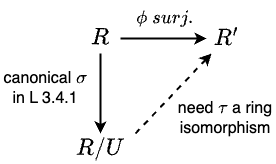
\includegraphics[width=0.4\textwidth]{Figures/Ring_1st_iso_black.png}
\end{center}
Define $\tau: R/U \rightarrow R'$ by $\tau(a+U)= \phi(a)$, this mapping lifts $a+U$ to preimage ``$a$" then applies $\phi$. As in the proof of first isomorphism theorem for groups, $\tau$ is well-defined, bijective, and a group homomorphism (under $+$); it remains to show $\tau$ splits over $\cdot$ \steezybreak\\
Let $a+U, b+U \in R/U$
\begin{align}
    \tau[(a+U)(b+U)]=\tau[ab+U]=\phi(ab)\underset{\substack{\uparrow \\ \phi \ ring \ hom.}}{=} \phi(a)\phi(b) =\tau[a+U]\tau[b+U]. \ \  \blacksquare \nonumber
\end{align}
    
\end{theorem}

\section{Ideal Theory}

\subsection*{Constructing Ideals} $U,V$ ideals in $R$
\begin{enumerate}
    \item $U\cap V < R$\steezybreak\\
    Check absorption: take $r\in R$, $x\in U\cap V$\\
    $rx\in U$ by absorption in $U$\\
    $rx\in V$ by absorption in $V$\\
    $\therefore$ $rx\in U\cap V$\\
    similarly $xr \in U \cap V$ \\
    $\therefore$ $U\cap V$ is an ideal.

    \item Recall that when you have $H,K$ subgroups in group $G$ then $HK<G \iff HK=KH$. Now consider $U,V$ ideals in $R$ (thinking of them as subgroups of $R$ under $+$) Lemma 2.5.1 says
    \begin{align}
        U+V<R \iff U+V=V+U \ \ \ \ \ (\text{Automatic in a ring which is abelian under }+) \nonumber
    \end{align}
    Checking absorption: take $r\in R$, $x\in U+V \ \ \implies \exists \ u\in U $ and $v\in V \ \ni x=u+v$
    \begin{align}
        rx=r(u+v)=\underset{\in U}{ru} + \underset{\in V}{rv} \in U+V \nonumber
    \end{align}
    similarly, $xr \in U+V$\\
    $\therefore$ $U+V$ is a two-sided ideal in $R$.
    \item Let $R$ comm. ring, $\forall \ a\in R, \ \ Ra=\{ra \ | \ r\in R\}$, $Ra$ is an ideal in $R$ called ``the ideal \textit{generated} by $a$"\\
    \textit{Proof:} Take $a\in R$, we will first show $Ra$ is a subgroup of $R$ under $+$ and then we will show it has the absorption property. First, note $0\cdot a=0\in Ra$ and $1\in R$, so $1\cdot a=a\in R$, so $R\neq \emptyset$ and Lemma 2.4.1 applies.\\
    \textbf{+ Closure:} Take $ra, \ sa \in Ra$
    \begin{align}
        ra+sa\underset{\substack{\uparrow \\ right \\dist. \\law}}{=}\underset{\substack{\in R \\ (+ closure)}}{(r+s)}a \in Ra \nonumber
    \end{align}
    \textbf{+ Inverses:} Take $ra$ as above, $\exists \ -ra$ because $ra\in R$
    \begin{align}
        -(ra)\underset{\substack{\uparrow \\ L3.2.1 (ii)}}{=} (-r)a\in Ra \ \ \ \ (\text{since }R \text{ contains the }+\text{ inv. ``}-r"\text{ for its elt. ``} r") \nonumber
    \end{align}
    $\therefore \ $ by Lemma 2.4.1 $Ra<R$ \\ \steezybreak
    \textbf{Absorption:} Take $x\in R$, $ra\in Ra$.
    \begin{align}
        (ra)x \underset{\substack{R \\ comm.}}{=} x(ra) \underset{assoc.}{=} \underset{\in R}{(xr)}a \in Ra \nonumber
    \end{align}
    $\therefore \ $ $Ra$ has the absorption property.  $\blacksquare$
\end{enumerate}\steezybreak
We know ``$0$" (+``$e$") is in every ideal. What about ``$1$" ($\ \cdot$ ``$e$")? \\ If $U$ is an ideal in $R$ and $1\in U$ then $\forall \ r \in R$, $r=r\cdot \underbrace{1}_{\in U} \in U$ by absorption. Which implies $R\subset U$, and since $U\subset R,  \ \ \implies \ \ U=R$ \\
\begin{tcolorbox}[width=5in, center=true]
\begin{center}
$\bigstar$: \ \ \ The only ideal containing $1$ is $R$.
\end{center}
\end{tcolorbox}
\begin{lemma}
    $R$ commutative ring and $R\neq \emptyset$.
    \begin{align}
        R \text{ is a field } &\iff \text{ the only ideals of }R \text{ are trivial.} \nonumber
    \end{align}
    \textit{Proof:}\\
    $\Rightarrow$: Assume $R$ is a field (comm. div. ring) and suppose $U$ is an ideal in $R$ with $U\neq \{0\}$ (we will show $U=R$). $U\neq \{0\} \ \implies  \ \exists \ u \in R \ni u\neq 0$, since $R$ is a division ring $\implies$ $\exists \ u^{-1}\in R$ but $1=\underset{\in U}{u}\cdot \underset{\in R}{u^{-1}}\in U$ by absorption. Therefore, $U=R$ by $\bigstar$. \\ \steezybreak
    $\Leftarrow$: Assume $\{0\}$ and $R$ are the only ideals in $R$. \\
    $R$ commutative, so it suffices to show that every non-zero element in $R$ has a multiplicative inverse (making $R$ a division ring). Take $a\in R \ni \ a\neq 0$, then $Ra$ is an ideal, so by our hypothesis $\implies$ $Ra=\{0\}$ or $Ra=R$. $Ra$ cannot be $\{0\}$ because $Ra$ contains $1\cdot a = a \neq 0$, so $Ra=R$. Therefore $\exists \ r \in R \ni ra = 1$ and $r$ is the required mult. inverse of $a$. \ \ \ $\blacksquare$ \\ 

    \noindent (Clarification: if $Ra=R$ that means every element of $R$ can be expressed as $ra$ for some $r\in R$, in particular, $1\in R$ can be expressed this way, and the $r$ that does this serves as the mult. inverse for $a$.)
\end{lemma}
\begin{example}
    The only ideals in $\Q, \R,$ and $\C$ are trivial (L3.5.1)
\end{example}
\begin{example}
    What are the ideals in $\Z$? Earlier we showed that $\forall \ n\in \Z$, $n\Z=\{ \text{ integer multiples of }n\}$ is an ideal in $\Z$. What other ideals in $\Z$ might there be? Ideals come from pool of subgroups of $\Z$
    \begin{align}
        \Z &\text{ is cyclic }: \ \ \Z=\langle 1 \rangle \nonumber \\
        1^0&=0 \nonumber \\
        1^1&=1 \nonumber \\
        1^2&=2 \nonumber \\
        1^{-2}&= (1^{-1})^2 = (-1)+(-1)=-2 \nonumber \\
        &\vdots \nonumber
    \end{align}
    every subgroup of a cyclic group is cyclic so ideals in $\Z$ have the form $\langle n \rangle$
    \begin{align}
        \langle n \rangle &= \{\cdots, -3n, -2n, -n, 0, n, 2n, 3n, \cdots\} = n\Z \nonumber
    \end{align}
    so $n\Z$'s account for all ideals in $\Z$. \\ \steezybreak 
    Note that $\langle n \rangle = \langle -n \rangle$ so it's customary to use the non-negative generator $\langle +n \rangle$.
\end{example}
\begin{definition}[Maximal Ideal]
    An ideal $M\neq R$ is \textit{maximal} if whenever an ideal $U$ satisfies $M\subseteq U \subseteq R$, either $M=U$ or $U=R$ \\ 
    
    \noindent (i.e. you can't slip a 3rd ideal strictly between $M$ and $R$)
\end{definition}
\begin{example}
    Consider $4\Z \varsubsetneqq 2\Z \varsubsetneqq \Z$, $4\Z$ is not maximal because we can slip $2\Z$ between $4\Z$ and $\Z$. What about $2\Z$? (we think its maximal) \\ \steezybreak
    Assume $2\Z \varsubsetneqq n\Z \ \implies$ $n\Z$ must have an odd integer
    \begin{align}
        &\implies \exists k \in \Z \ni 2k+1 \in n\Z \nonumber \\
        2k \in 2\Z \subset n\Z &\implies 2k \in n\Z < \Z \nonumber \\
        &\implies -2k \in n\Z \nonumber \\
        (2k+1)+&(-2k) \in n\Z  \nonumber \\
        &\implies 1\in n\Z \nonumber \\
        &\implies n\Z = \Z \ \ \ (\text{ by }\bigstar) \nonumber
    \end{align}
    so $2\Z$ is maximal in $\Z$.
\end{example}
\begin{example}
    What about $3\Z$? If $3\Z \varsubsetneqq n\Z \subseteq \Z$ then
    \begin{align}
        3\Z \varsubsetneqq n\Z &\implies \ n\Z \text{ contains a member of the form }3k+1 \text{ or } 3k+2 \text{ for some }k\in \Z \nonumber \\
        \text{Suppose }3k+1 \in n\Z &\implies 3k+1 + (-3k) \in n\Z  \nonumber \\
        &\implies 1 \in n\Z \nonumber \\
        &\implies n\Z = R \nonumber \\
        \text{Now, suppose }3k+2 \in n\Z &\implies -(3k+2)\in n\Z \nonumber \\
        &\implies 3k+1+[-(3k+2)]\in n\Z \nonumber \\
        &\implies 1 \in n\Z \nonumber \\
        \therefore \ n\Z &= \Z \nonumber \\
        \therefore \ 3\Z &\text{ is maximal. } \nonumber
    \end{align}
    \begin{figure}[h!]
        \centering
        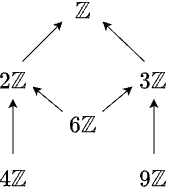
\includegraphics[width=0.3\linewidth]{Figures/Maximal_Ideals_Factor_Graph_thing.png}
    \end{figure}
\end{example}

\begin{proposition}
    Given $n\in \Z^{+}$ \\ $n\Z$ is maximal in $\Z$ $\iff \ n$ is prime. \\
    \textit{Proof: } \\ \steezybreak
    $\Leftarrow$ : Suppose $n=p$ is prime and suppose $p\Z \varsubsetneqq \underbrace{m\Z}_{ideal} \subseteq \Z$
    \begin{align}
        &p\in m\Z \implies \exists \ k \in \Z \ni \ p=mk \ \ \ \ (p\text{ prime so divisor } m \text{ can only be }1 \text{ or }p) \nonumber \\
        &\text{Since }m\Z \neq p\Z, \ m\text{ can't be }p, \text{ so }m=1. \nonumber \\
        & \text{Now, }1\Z=\Z, \ \therefore \ p\Z \varsubsetneqq 1\Z \subseteq \Z \nonumber \\
        &\text{So, }m\Z=\Z \ \therefore \ p\Z \text{ is maximal.} \nonumber
    \end{align}
    $\Rightarrow$: Assume $n\Z$ is maximal and suppose $n=ab$ where $a,b\in \Z^{+}$. Consider ideal $a\Z$, any multiple of $n$ is also a multiple of $a$, so
    \begin{align}
        \underbrace{n\Z}_{maximal} &\subseteq a\Z \subseteq \Z \nonumber
    \end{align}
    $n\Z$ maximal $\implies$ either $a\Z=n\Z$ or $a\Z=\Z$ \\ \steezybreak
    If $a\Z=\underset{\substack{\uparrow \\ 1\in }}{\Z}$, then $\exists \ k\in \Z \ni ak = 1$, since $a$ and $k$ are integers $\implies a=k=1 \ \implies a=1$ so $b=b\cdot 1 = b\cdot a = n$, so in this case, $n$ factors only as $1\cdot n$. \\ \steezybreak
    If $a \underset{\substack{\uparrow \\ 1 \in}}{\Z} = n\Z$, then $\exists \ k\in \Z \ni a\cdot 1 =nk, \ \implies$ $a$ can be written in the form $a=nk$.
    \begin{align}
        n&= ab = nkb \nonumber
    \end{align}
    applying cancellation in integral domain $\Z \ \ \implies \ 1=kb$, now since $k,\ b$ are integers and $b$ positive $\implies \ \ k=b=1$, so we have $a\cdot 1 = a = ab=n$. So again, $n$ can only be factored as $n\cdot 1$. \\ \steezybreak
    $\therefore$ $ n$ is prime since it's only possible divisors are $n$ and $1$. $\blacksquare$
\end{proposition}

\setcounter{dummy}{0}
\begin{theorem}
    Suppose $R$ is a commutative ring with $1$ and $M$ is an ideal of $R$ with $M\neq R$, then:
    \begin{align}
        M \text{ is maximal } \iff R/M \text{ is a field.} \nonumber
    \end{align}
    \textit{Proof: }\\
    $\Leftarrow$: Assume $R/M$ is a field. \\
    Suppose $V$ is an ideal $\ni$ $M\varsubsetneqq V \subseteq R$ (Show $V=R$)
    \begin{align}
        M \varsubsetneqq V \implies \ \exists \ x \in V \ni x\not \in M \nonumber
    \end{align}
    Consider $x$'s coset in $R/M$:
    \begin{center}
    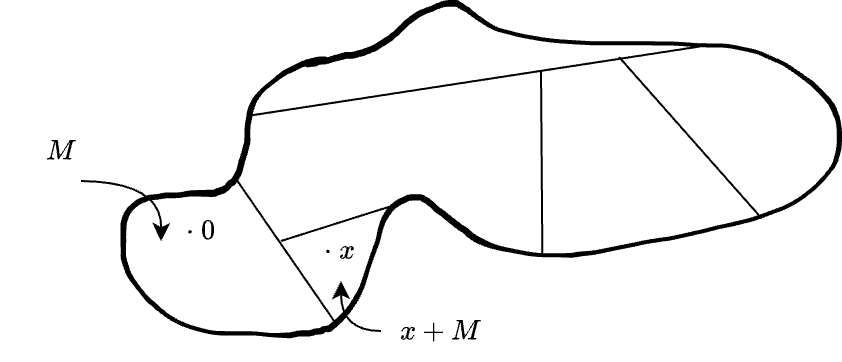
\includegraphics[width=0.65\textwidth]{Figures/x_coset_in_R_M.png} \\ 
    \end{center}
    Recall that $a+U=b+U \iff a-b\in U$ \\
    Since $x\not \in M \implies \ x+M$ is non-zero (i.e. it's not $0+M$) in the field $R/M$. So it has a multiplicative inverse in $R/M$, call it $y+M$
    \begin{align}
        1+M &= (x+M)(y+M)=xy+M\nonumber \\
        &\therefore 1-xy \in M \nonumber
    \end{align}
    \begin{align}
        1&= \underset{\in M \subset V}{(1-xy)}+\underset{\underbrace{\substack{\uparrow\uparrow\\x \in V y\in R}}_{\in V \text{ by abs.}}}{xy} \in V \text{ by }+ \text{ closure.} \nonumber \\
        \therefore & \ V=R \ \ \ (\text{ by }\bigstar) \text{ and so } M \text{ is maximal.} \nonumber
    \end{align}

    \begin{tcolorbox}[width=5in, center=true]
    \begin{center}
        \textbf{Side Notes}
    \end{center}
    $H<G$
    \begin{center}
        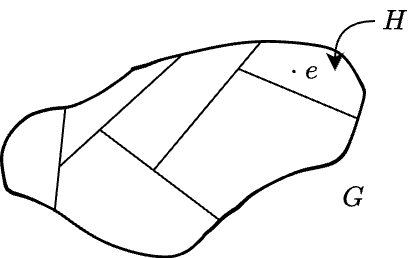
\includegraphics[width=0.45\textwidth]{Figures/subgroup_idk.png}
    \end{center}
    \begin{align}
        [a]=[b]\iff a\sim b \iff a \equiv b \mod H \iff ab^{-1}\in H \nonumber
    \end{align}
    \begin{center}
    \begin{tcolorbox}[width=0.4\textwidth]
        $Ha = Hb \iff ab^{-1}\in H$
    \end{tcolorbox}
    \end{center}
    Ideal $M<R$
    \begin{center}
        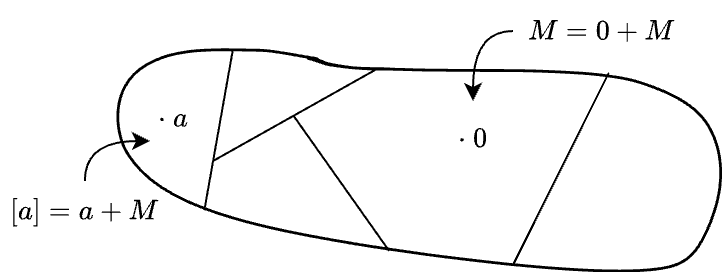
\includegraphics[width=0.65\textwidth]{Figures/Ideal_idk.png}
    \end{center}
    \begin{align}
        [a]=[b]\iff a\equiv b \mod M \iff a-b\in M \nonumber
    \end{align}
    \begin{center}
    \begin{tcolorbox}[width=0.5\textwidth]
        $a+M=b+M \iff a-b \in M$
    \end{tcolorbox}
    \end{center}
    \end{tcolorbox}
    \noindent $\Rightarrow$:  Assume $M$ is maximal. \\
    $M$ ideal $\implies$ $R/M$ is a ring by Lemma 3.4.1. What's more $R$ commutative $\implies$ $R/M$ commutative meaning $\forall \ a,b \in R$ we have 
    \begin{align}
        (a+M)(b+M) \ \ & \ \ \ \ = \ \ \ ab+M \nonumber\\
        &\underset{R \text{ comm.}}{=}ba+M \nonumber \\
        & \ \ \ \ = \ \ \ (b+M)(a+M) \nonumber
    \end{align}
    It remains to show that $R/M$ has multiplicative inverses for its non-zero elements. \\ \steezybreak
    \noindent Take $x+M \in R/M$ non-zero
    \begin{center}
        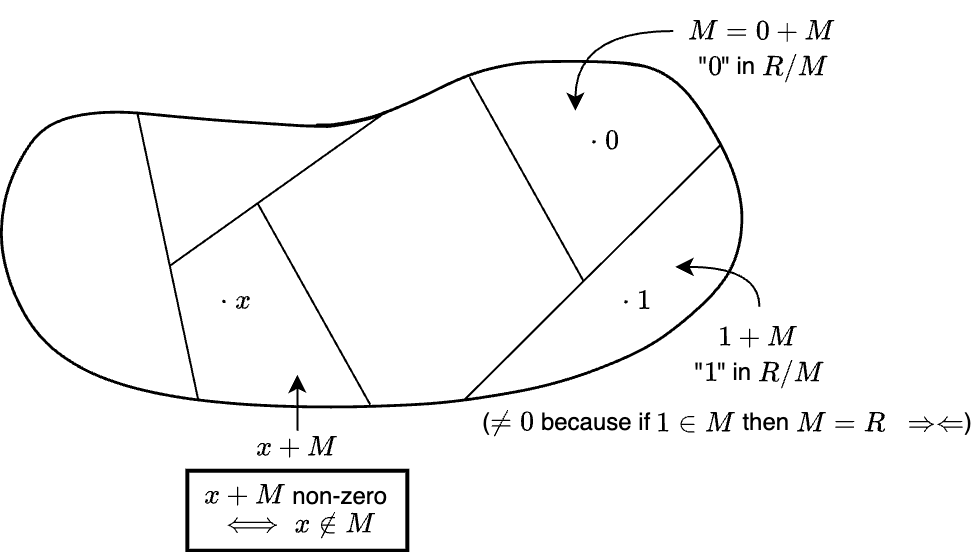
\includegraphics[width=0.75\textwidth]{Figures/M_maximal_idk.png}
    \end{center}
    We will use $x$ to construct an ideal, (remember $Rx$ is the ideal generated by $x$ and the sum of two ideals is an ideal)
    \begin{align}
        &Rx+M \nonumber \\
        x&= 1\cdot x + 0 \in Rx + M \nonumber\\
    \text{furthermore,}& \nonumber \\
        \forall m \in M \ \ m &= 0\cdot x + m \in Rx+M \nonumber
    \end{align}
    So,
    \begin{align}
        \underset{x\not\in}{M} \varsubsetneqq \underset{x\in}{Rx+M} \subset R \nonumber
    \end{align}
    But $M$ was assumed maximal $\implies Rx+M = R$. Now, since $1\in R$,
    \begin{align}
        \exists \ \bar{r} \in R \text{ and } \bar{m}\in M \ni 1&=\bar{r}x+\bar{m} \nonumber \\
        \implies 1-\bar{r}x &= \bar{m} \nonumber \\
        \implies 1-\bar{r}x &\in M \nonumber \\
        \implies 1+M &= \bar{r}x+M \nonumber \\
        \implies 1+M &= (\bar{r}+M)(x+M) \nonumber 
    \end{align}
    So $(\bar{r}+M)$ is $(x+M)^{-1}$ in $R/M$. \\
    $\therefore$ $\ R/M$ is a field. \ \ \ \ $\blacksquare$
\end{theorem}
\newpage 
\subsection{$\Z_n$ Recap}
\begin{align}
    \Z_n = \{0,1,\cdots , n-1\} \text{ under  }  +,\ \cdot \ \ (\mod n) \nonumber
\end{align}
$\Z$ has ideal $n\Z$, so $\Z/n\Z$ is a ring (commutative).

\begin{align}
    \Z/n\Z = \{\underbrace{0+n\Z}_{[0]}, \underbrace{1+n\Z}_{[1]}, \underbrace{2+n\Z}_{[2]}, \cdots , \underbrace{(n-1)+n\Z}_{[n-1]}\} \nonumber
\end{align}

\begin{align}
    \Z/n\Z &\approx \Z_n \ \ \ \ \text{    via a simple name change:} \nonumber \\
    [x] \ \ &\leftrightarrow x \ \ \ \ \text{    so }\Z_n \text{ has the ring structure of }\Z/n\Z \nonumber
\end{align}
\begin{align}
    \Z_n \approx \Z/n\Z \text{ is a field } &\iff n\Z \text{ is maximal} \nonumber \\
    &\iff \ n \text{ is prime} \nonumber
\end{align}
\begin{align}
    &\Z_2, \Z_3, \Z_5, \cdots , \Z_p, \cdots \ \ &\text{ fields}\nonumber \\
    &\Z_4, \Z_6, \Z_8, \cdots , \Z_{\text{composite}}, \cdots \ \ &\text{ basic comm. rings, all have zero divisors} \nonumber
\end{align}
\begin{example}
    Find the multiplicative inverse of $28$ in $\Z_{53}$. \\ \steezybreak
    
    \begin{align}
        \text{We need } x\in \{0,1,\cdots, 52\} &\ni 28\cdot x \equiv 1 \mod 53 \nonumber \\
        &\iff 28x-1=53k \ \ \ \text{     for some }k\in \Z \nonumber \\
        &\iff \underset{\substack{\uparrow \ \ \ \ \ \ \ \  \uparrow \ \ \ \ \ \ \\ Rel. \ prime \ \ \ }}{28x+53(-k)}=1 \nonumber
    \end{align}

    \begin{align}
        53&= \overset{\substack{q \\ \ }}{\colorbox{green}{1}}\cdot 28 + \overset{\substack{r \\ \ }}{25} \nonumber \\
        28&= \colorbox{green}{1}\cdot 25 + 3 \nonumber \\
        25&= \colorbox{green}{8}\cdot 3 + 1 \nonumber \\
        3&= 3 \cdot 1 + 0 \nonumber
    \end{align}
    \begin{align}
        \underbrace{\begin{pmatrix}
            0&1 \\
            1 & -8
        \end{pmatrix}
        \begin{pmatrix}
            0&1 \\
            1 & -1
        \end{pmatrix}}_{\searrow}
        \begin{pmatrix}
            0&1 \\
            1 & -1
        \end{pmatrix}& \nonumber \\
        \begin{pmatrix}
            1&-1 \\
            -8 & 9
        \end{pmatrix}
        \begin{pmatrix}
            0&1 \\
            1 & -1
        \end{pmatrix}&= \begin{pmatrix}
            *&* \\
            9 & -17
        \end{pmatrix} \nonumber
    \end{align}
    $\therefore \ (9)53+(-17)28 = 1$ \\ \steezybreak
    
    \noindent Pass to $\Z_{53}$ \ \ $-17+53=36$ \\ \steezybreak
    
    \noindent $(36)(28)=1$ in $\Z_{53}$
\end{example} 
\newpage 

\section{The Field of Fractions (Quotients) of an Integral Domain}
\begin{theorem}
    Every integral domain can be extended to a field. \\
    \textit{Proof}: This proof is a construction. \steezybreak \\
    Let $D$ be an integral domain, form the set $D\times (D-\{0\})=\{(a,b) \ | \ a,b\in D, \ b\neq 0\}$ \steezybreak \\
    Now define relation $\sim$ on $D\times (D-\{0\})$
    \begin{align}
        (a,b)\sim (c,d) &\iff ad=bc \nonumber
    \end{align}
    $\sim$ is an equivalence relation: \\
    \noindent \textbf{Reflexive}: \\ 
    \indent $\ \ (a,b)\sim (a,b)$ because $ab=ba$ (integral domains are commutative)\\
    \noindent \textbf{Symmetric}: 
    \begin{align}
        (a,b)\sim (c,d) \implies ad=bc &\overset{D \  comm.}{\implies} da=cb \nonumber \\
        & \ \implies cb=da \ \ \ \ \ \ \ \ (\text{symmetry of }``=") \nonumber \\
        & \ \implies (c,d)\sim (a,b) \nonumber
    \end{align} \\
    \noindent \textbf{Transitive}: \\
    Assume $(a,b)\sim (c,d)$ and $(c,d)\sim (e,f)$
    \begin{align}
        (a,b)&\sim (c,d) \implies ad=bc \nonumber \\
        (c,d)&\sim (e,f) \implies cf=de \nonumber \\
        &\implies adf= bcf \nonumber \\
        &\implies a\not d f = b\not d e  \ \ \ \ \ (D \text{ int. domain }\iff \text{ cancellation of non-zero elts. holds in }D)\nonumber \\
        &\implies af=be \ \implies (a,b)\sim (e,f) \nonumber
    \end{align}
    \\

    \noindent Denote the equivalence class of $(a,b)$ by $\frac{a}{b}$ \steezybreak \\
    Let $F=\{\frac{a}{b} \ | \ a,b\in D, \  b\neq 0\} = \{\text{ equivalence classes under }\sim \text{ in }D\times (D-\{0\})\}$
    \begin{tcolorbox}
        \begin{center}
            \textbf{Pause proof for a moment for an aside:}
        \end{center}
        Two equivalence classes are either $\underset{\substack{\Updownarrow \\ \text{Reps are related}}}{\text{identical}}$ or $\underset{\substack{\Updownarrow \\ \text{Reps are unrelated} }}{\text{disjoint}}$\\
        So 
        \begin{align}
            \frac{a}{b}=\frac{c}{d} &\iff (a,b)\sim (c,d) \nonumber \\
            &\iff ad = bc \nonumber
        \end{align}
        So in effect, you can tell if two fractions are equal by ``cross multiplying".
        \begin{center}
            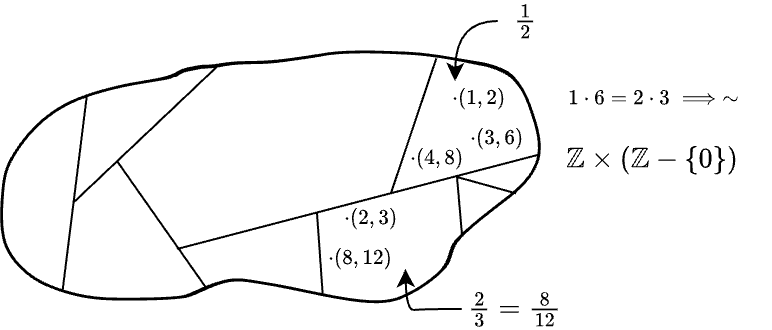
\includegraphics[width=0.75\textwidth]{Figures/quotient_equiv_classes.png}
        \end{center}
        \begin{center}
            \textbf{Ok, back to the proof!}
        \end{center}
    \end{tcolorbox}
    \noindent It remains to show that $F$ is a \textul{field}. \\ 
    Define $+$ on $F$ by
    \begin{align}
        \frac{a}{b}+\frac{c}{d} = \frac{ad+bc}{bd} \nonumber
    \end{align}
    Is this operation well-defined? Suppose $\frac{a}{b}$ and $\frac{a'}{b'}$ name the same class, and $\frac{c}{d}$ and $\frac{c'}{d'}$ name the same class
    \begin{align}
        \underset{\substack{\nwarrow \ \ \ \ \ \ \ \nearrow \\ \text{does }+\text{ give the same class?}}}{\underbrace{\frac{a}{b}+\frac{c}{d}} \ \ \ \ \ \ \underbrace{\frac{a'}{b'}+\frac{c'}{d'}}} \nonumber
    \end{align}
    User cross multiplying criteria \steezybreak \\
    We know $ab'=ba'$ and $cd'=dc'$
    \begin{align}
        \frac{ad+bc}{bd} = \frac{a'd'+b'c'}{b'd'} \iff (ad+bc)b'd' = bd(a'd'+b'c') \nonumber
    \end{align}
    So we must show $(ad+bc)b'd' = bd(a'd'+b'c')$
    \begin{align}
        (ad+bc)b'd' &= adb'd'+bcb'd' \nonumber \\
        &= ba'dd' + bb'dc' \nonumber \\
        &= bd(a'd'+b'c')\nonumber
    \end{align}
    $\therefore \ +$ is well defined. \steezybreak \\
    \newpage
    Next we will show $F$ is an abelian group under the $+$ we just defined. \\
    \noindent \textbf{$+$ Closure}: \\
    \begin{align}
        \frac{a}{b}+\frac{c}{d} = \frac{\overbrace{ad+bc}^{\in D}}{\underbrace{bd}_{\neq 0, \ \ \in D}} \in F \ \ \ \ \ \ (bd\neq 0\text{ because }b\neq 0, \ d\neq 0 \ \ \text{ and }D \text{ is an integral domain}) \nonumber
    \end{align}\\
    \noindent \textbf{$+$ Associative}: \\
    \begin{align}
        \left(\frac{a}{b}+\frac{c}{d}\right)+\frac{e}{f} &= \frac{ad+bc}{bd} + \frac{e}{f} \nonumber \\
        &= \frac{(ad+bc)f+(bd)e}{(bd)f} \nonumber \\
        &= \frac{a(df)+(bcf+bde)}{b(df)} \ \ \ \ \ \  \ \ (\text{L dist. and assoc. in }D) \nonumber \\
        &= \frac{a(df)+b(cf+de)}{b(df)} \nonumber \\
        &= \frac{a}{b} + \frac{cf+de}{df} \nonumber \\
        &= \frac{a}{b}+\left(\frac{c}{d}+\frac{e}{f}\right) \ . \nonumber
    \end{align}\\
    \noindent \textbf{$+$ Abelian}: \\
    \begin{align}
        \frac{a}{b}+\frac{c}{d}&= \frac{ad+bc}{bd}\nonumber \\
        &= \frac{da+cb}{db} \ \ \ \ \ (D \text{ comm.}) \nonumber \\
        &= \frac{cb+da}{db} \ \ \ \ \ (D \text{ abelian under }+) \nonumber \\
        &= \frac{c}{d}+\frac{a}{b} \ . \nonumber
    \end{align}\\
    \noindent \textbf{$+$ Identity ($\exists$ ``$0$" )}: \\
    \begin{align}
        \frac{a}{b}+\frac{0}{1} &= \frac{a\cdot 1 + b\cdot 0}{b\cdot 1} \nonumber \\
        &= \frac{a}{b} \nonumber
    \end{align}
    So we have a ``$0$" it is $\frac{0}{1}$.\\
    \noindent \textbf{$+$ Inverses}: \\ 
    \begin{align}
        \frac{a}{b}+\frac{(-a)}{b} = \frac{ab+b(-a)}{b^2} &= \frac{ab+[-(ab)]}{b^2} \nonumber \\
        &= \frac{0}{b^2} = \frac{0}{1} \ \ \ \ \ \ \ \ (\text{ Because }0\cdot 1 = b^2 \cdot 0 = 0) \nonumber
    \end{align}
    So $-\frac{a}{b}$ is $\frac{(-a)}{b}$
    \steezybreak \\
    So far, $F$ is an abelian group under $+$.  \steezybreak \\
    For $F$ to become a field we need to define a multiplication $\cdot$ for elements in $F$ and show 1) $\cdot$ closure, 2) $\cdot$ associativity, 3) $\cdot$ commutativity, 4) two distribution (left and right) laws for the $\cdot$, 5) the existence of a multiplicative identity, and 6) the existence of inverses under $\cdot$ \steezybreak \\
    Define multiplication on $F$ for $\frac{a}{b}, \ \frac{c}{d}$
    \begin{align}
        \frac{a}{b} \cdot \frac{c}{d}&= \frac{ac}{bd} \nonumber
    \end{align}
    Is it well defined? If $\frac{a}{b}=\frac{a'}{b'}$ and $\frac{c}{d}=\frac{c'}{d'}$ is $\frac{ac}{bd}=\frac{a'c'}{b'd'}$? Show $acb'd'=bda'c'$:
    \begin{align}
        acb'd'&\underset{\substack{\uparrow \\ ab'=ba'}}{=}ba'cd'\underset{\substack{\uparrow \\ dc'=d'c}}{=}ba'dc'=bda'c'\nonumber 
    \end{align}
    $\therefore \ $ cross multiplying criteria says YES! well defined.

    \noindent \textbf{$\cdot$ Closure}: \\
    \begin{align}
        \underset{\substack{\uparrow \\ \neq 0}}{\frac{a}{b}}\cdot  \underset{\substack{\uparrow \\ \neq 0}}{\frac{c}{d}} &= \underset{\substack{\uparrow \\ \neq 0, \in D}}{\frac{\overset{\substack{\in D \\ \downarrow}}{ab}}{cd}}\nonumber
    \end{align}
    \noindent \textbf{$\cdot$ Associative}: \\
    \begin{align}
        \left(\frac{a}{b}\cdot \frac{c}{d} \right) \cdot \frac{e}{f} &= \frac{a\cdot c}{bd} \cdot \frac{e}{f}\nonumber \\
        &= \frac{(ac)e}{(bd)f}\nonumber \\
        &= \frac{a(ce)}{b(df)} \nonumber \\
        &= \frac{a}{b}\cdot \frac{ce}{df} \nonumber \\
        &= \frac{a}{b} \cdot \left(\frac{c}{d}\cdot \frac{e}{f}\right) \nonumber
    \end{align}
    \noindent \textbf{$\cdot$ Commutative}: \\
    \begin{align}
        \frac{a}{b}\cdot \frac{c}{d}&= \frac{ac}{bd} \nonumber \\
        &= \frac{ca}{db} \ \ \ \ \ (D\text{ comm.}) \nonumber \\
        &= \frac{c}{d}\cdot \frac{a}{b} \nonumber
    \end{align}
    \noindent \textbf{$\cdot$ Distribution Laws}: \\
    \begin{enumerate}
        \item \begin{align}
            \frac{a}{b}\left(\frac{c}{d}+\frac{e}{f}\right) &= \frac{a(cf+de)}{b(df)}\nonumber \\
            &= \frac{acf+ade}{bdf} \nonumber
        \end{align}
        on the other hand,
        \begin{align}
            \frac{a}{b}\cdot \frac{c}{d}+\frac{a}{b}\cdot \frac{e}{f} &= \frac{ac}{bd}+\frac{ae}{bf} \nonumber \\
            &= \frac{acbf+bdae}{bdbf} \nonumber \\
            &= \frac{acf+ade}{bdf} \ \ \ \ \ \ \ (\text{ by cross mult. criteria}) \nonumber
        \end{align}
        \item 
        \begin{align}
            \left( \frac{c}{d}+\frac{e}{f} \right)\frac{a}{b} &= \frac{a}{b}\left(\frac{c}{d}+\frac{e}{f}\right) \nonumber \\
            &= \frac{a}{b}\cdot \frac{c}{d} + \frac{a}{b}\cdot \frac{e}{f} \nonumber \\
            &= \frac{c}{d}\cdot \frac{a}{b} + \frac{e}{f} \cdot \frac{a}{b} \nonumber 
        \end{align}
    \end{enumerate}
    \noindent \textbf{$\cdot$ Identity ($\exists$ ``$1$")}: \\
    \begin{align}
        \overset{\substack{\text{mult ID in }D \\ \searrow \\}}{\frac{a}{b}\cdot \frac{1}{1}} &= \frac{a\cdot 1}{b \cdot 1} \nonumber \\
        &= \frac{a}{b} \nonumber
    \end{align}
    \noindent \textbf{$\cdot$ Inverses}: \\
    Suppose $\frac{a}{b}\neq \frac{0}{1}$ well then $a\cdot 1 \neq b\cdot 0$ so $a\neq 0$, thus $\frac{b}{a}\in F$ and 
    \begin{align}
        \frac{a}{b}\cdot \frac{b}{a} &= \frac{ab}{ba} = \frac{1}{1} \ \ \ \ \ (\text{by cross mult. criteria in }D \text{ comm.}) \nonumber
    \end{align}
    $\therefore  \ F$ is a field. \ \ \  $\blacksquare$
\end{theorem}

In the theorem above (Thm 3.6.1), $F$ \textit{extends} $D \ \ \implies$ $\exists$ an injective ring homomorphism from $D$ into $F$. \\
\begin{definition}[Embedding of $D$ into $F$]
    \label{defn:embeddingofD}
    Given $D$ integral domain, and $F$ as constructed above from $D$, we define an injective ring homomorphism $\phi: D \rightarrow F$ by
    \begin{align}
        \phi(a) &= \frac{a}{1} \nonumber \\ 
        \phi(a+b) &= \frac{a+b}{1} = \frac{a\cdot 1+b\cdot 1}{1\cdot 1} = \frac{a}{1}+\frac{b}{1} = \phi(a)+\phi(b) \nonumber \\
        \phi(ab) &= \frac{ab}{1} = \frac{ab}{1\cdot 1} = \frac{a}{1}\cdot \frac{b}{1} = \phi(a)\cdot \phi(b) \nonumber 
    \end{align}
    If $a\neq b$ then $\frac{a}{1} \neq \frac{b}{1}$ because $b\cdot 1 \neq a \cdot 1$ \\
    $\therefore$ $\phi(a)\neq \phi(b)$, so $\phi$ is injective.
\end{definition}

\begin{definition}[Field of Fractions (of an Integral Domain)]
Given integral domain $D$, then the field $F$, as constructed in Theorem 3.6.1, is known as the \textit{Field of Fractions} of $D$ and $D$ is said to be \textit{embedded} in $F$ by $\phi$ from Definition \ref{defn:embeddingofD}.
\end{definition}
\newpage
\subsection{Leftover questions from Theorem 3.6.1} 

\begin{align}
    &F = \left\{\frac{a}{b} \ | \ a,b\in D, \  b\neq 0 \right\} \nonumber \\
    &\vert \nonumber \\ 
    &D \nonumber \\
    & \nonumber \\
    D &\times (D-\{ 0 \}) \nonumber \\
    \frac{a}{b} &= \frac{c}{d} \iff bc=ad \nonumber
\end{align}

\begin{enumerate}
    \item Why can't we include $0$ as a denominator? Let's try leaving it in: use $D\times D$, then the class of $(1,0)$ is denoted $\frac{1}{0}$
    \begin{align}
        &\frac{1}{0}, \text{ so }\frac{1}{0}\in F \nonumber \\
        \frac{0}{1} &= \frac{1}{0}\cdot \frac{0}{1} = \frac{1\cdot 0}{0\cdot 1} = \frac{0}{0} \underset{\substack{\text{by cross} \\ \text{mult criteria}}}{=}\frac{1}{1} \nonumber
    \end{align}
    So in $F$ we have $0=1$ or $+ \text{ identity}=\text{mult. identity}$, Then
    \begin{align}
        \forall &r \in F \ \text{ we have} \nonumber \\
        r &= r\cdot 1 = r\cdot 0 \underset{L \ 3.2.1}{=} 0 \implies F = \{0\} \text{ \ \ \  (Trivial!)} \nonumber
    \end{align}
    $\therefore$ if $R$ is non-trivial then it must have the separation between $+$ and $\cdot \ \text{ID}$. So $1\neq 0$ and $R$ cannot have a $0$ inverse among its elements. (Because existence of $0^{-1} \implies 1=0 \Rightarrow \Leftarrow$)
    \item Can we build $\R$ from $\Q$ using a similar process? Getting $\Q$ doesn't give you all of $\R$: \\ \steezybreak
    Suppose $\sqrt{2} \in \Q$
    \begin{align}
        \frac{\sqrt{2}}{1}=\frac{a}{b} &\implies \sqrt{2}b=a \nonumber \\
        &\implies 2b^2 = a^2 \nonumber
    \end{align}
    $a$ and $b$ have prime factorizations \\
    Count the number of $2$'s in prime factorizations of $2b^2$ and $a^2$ \\
    $a^2$ has an even number of $2$'s in factorization ($2k$ where $k$ is number in $a$'s factorization) \\
    $b^2$ has an even number by a similar argument \\
    so $2b^2$ has an odd number in its factorization! So $2b^2 \neq a^2$ $\Rightarrow \Leftarrow$ \\
    $\therefore \sqrt{2} \not \in \Q$ \\
    By a similar argument, in general, $\sqrt{p} \not \in \Q$ for $p$ prime. \\
    Algebra $+$ Analysis $\implies \ \R $ \\
    Algebra is the skeleton, Analysis is ethereal. 
\end{enumerate}

\section{Polynomial Rings}
In the next two sections,  we will present some results from both sections 3.7 and 3.9 of Herstein's book, to be consistent with the theorem and lemma numbers in Herstein's text you may notice the numbers suddenly jump from 3.7.x to 3.9.x, this is intentional. I just want it to be easy for you to reference the relevant sections in Herstein's text if you are following along with his book as you read ours. \\
\newpage 
\noindent In the definition below $X$ is a formal placeholder
\begin{definition}[Ring of Polynomials in $X$ over $F$]
    The \textit{Ring of Polynomials} in $X$ over $F$, denoted $F[X]$ is defined as follows
    \begin{align}
        F[X]= \{a_0 + a_1X + a_2X^2 + a_3X^3 + \cdots + a_m X^m \ | \ a_i \in F \text{ for } 0\leq i \leq m, \ \ m \text{ any non-zero integer}\} \nonumber
    \end{align}
    $a_i$'s are coefficients.
\end{definition}

\noindent For the following three definitions suppose that
\begin{align}
    p(x)&= a_0 + a_1x + \cdots + a_mx^m \in F[x] \nonumber \\
    \text{and } \ \ q(x)&= b_0+b_1x+\cdots + b_n x^n \in F[x] \nonumber
\end{align}

\begin{definition}[Equality of Polynomials]
    \begin{align}
        p(x)=q(x) \iff b_i = a_i \ \forall \ i \geq 0 \nonumber 
    \end{align}
    That is, polynomials are equal if and only if their corresponding coefficients agree.
\end{definition}

\begin{definition}[Sum of Polynomials]
    \begin{align}
        (p+q)(x)= p(x)+q(x) \underset{defn.}{=}c_0 + c_1x + \cdots + c_t x^t \nonumber
    \end{align}
    where $c_i = a_i+b_i$ $\forall \ i\geq 0$ (Add like terms).
\end{definition}

\begin{definition}[Product of Polynomials]
    \begin{align}
        (pq)(x) &= \underbrace{p(x)\cdot q(x)}_{\text{notation}} \nonumber \\ 
        &\underset{defn.}{=} c_0 + c_1x + c_2x^2 + \cdots + c_kx^k \nonumber 
    \end{align}
    Where 
    \begin{align}
        c_i &= a_i b_0 + a_{i-1}b_1 + a_{i-2}b_{2} + \cdots + a_1b_{i-1} + a_0b_i \  \forall  \ i \geq 0 \nonumber \\
        \ \nonumber \\
        c_0 &= a_0b_0   \nonumber \\
        c_1 &= a_1b_0 + a_0b_1 \ \ \ \ \ \ \ \ \ \ \ \ \ (\text{Distribute } x^\alpha \cdot x^\beta = x^{\alpha + \beta}) \nonumber \\
        &\vdots \nonumber
    \end{align}
    and so on, 
\end{definition}

\begin{example}
    \begin{align}
        &(a_0 + a_1x + a_2x^2)(b_0 + b_1x) \nonumber  \\
        &= a_0b_0 + a_0b_1x + a_1x b_0 + a_1xb_1x + a_2x^2b_0 + a_2x^2+b_1x \nonumber \\
        &= \underbrace{(a_0b_0)}_{c_0} + \underbrace{(a_0b_1+a_1b_0)}_{c_1}x + \underbrace{(a_1b_1+a_2b_0)}_{c_2}x^2+ \underbrace{(a_2b_1)}_{c_3}x^3 \nonumber
    \end{align}
    Note, in this example, if we want to write things out thoroughly for $c_2$ and $c_3$ we have:
    \begin{align}
        c_2 &= \colorbox{green}{$a_2b_0 + a_1b_1$}+\underbrace{a_0b_2}_{=0} \nonumber \\
        c_3 &= \underbrace{a_3b_0}_{=0}+ \colorbox{green}{$a_2b_1$}+ \underbrace{a_1b_2}_{=0} + \underbrace{a_0b_3}_{=0} \nonumber
    \end{align}
\end{example}
$F[x]$ is a commutative ring under $+$ and $\cdot$ as defined above. \\ 
\noindent The ``$0$'' is $f(x) = 0_F+ 0x + 0x^2 + \cdots  $ \\
\noindent The ``$1$'' is $g(x) = 1_F$ where $1_F$ is the multiplicative identity in $F$. \\
\begin{definition}[Degree (of a Polynomial)]
    Let $f(x) \in F[x]$ 
    \begin{enumerate}
        \item the \textit{degree} of $f$ is the largest integer $i$ for which $a_i \neq 0$ \\ \steezybreak 
        (So $f(x) = a_0 + a_1x + a_2x^2 + \cdots a_mx^m$ and $a_m \neq 0 \ \implies \deg f = m$ )
        \item ``$0$'' ($f(x)=0_F$) is said to be ``without degree''.
        \item $f(x)\in F[x]$ is constant $\iff$ $f$ has degree $0$.
        \begin{align}
            f(x) &= \underbrace{a_0}_{\neq 0} x^0 = a_0 \in F \nonumber
        \end{align}
        The constants in $F[x]$ are the non-zero field elements.
    \end{enumerate}
\end{definition}
Here's a quick example to clarify the last two parts of the definition above, in $\R[x]$
\begin{align}
    f(x)&=5 \ \ \ \leftarrow \text{ has degree }0 \nonumber \\
    g(x)&=0 \ \ \ \leftarrow \text{ is without degree}. \nonumber
\end{align}

% Artificially bump section number ahead!
\setcounter{section}{8}
\begin{tcolorbox}
    We are briefly going to jump ahead to some section 3.9 material from Herstein's book, and then we will return to 3.7 material, I hope this isn't too confusing...
\end{tcolorbox}
\section{Rational Functions in $X$ over $F$ and Euclidean Rings}
\begin{lemma}
    $f,g$ non-zero in $F[x]$
    \begin{align}
        \deg(fg)= \deg(f)+\deg(g) \nonumber
    \end{align}
    \textit{Proof:} \\
    \noindent Suppose 
    \begin{align}
        f(x)= a_0 +a_1x+\cdots + a_mx^m \text{ where } a_m \neq 0 \nonumber \\
        g(x)= b_0 +b_1x + \cdots + b_nx^n \text{ where } b_n\neq 0 \nonumber
    \end{align}

    \begin{align}
        f(x)g(x) &= c_0 + c_1x + \cdots c_kx^k \nonumber
    \end{align}
    where $c_i = a_ib_0 + a_{i-1}b_1 + \cdots a_1b_{i-1} + a_0 b_i$. \\
    \noindent we must show $c_{m+n}\neq 0$ and $c_i = 0 \ \forall \ i >m+n$
    \begin{align}
        c_{m+n} &= a_{m+n} b_0 + a_{m+n-1}b_1 + \underbrace{\cdots}_{a_mb_n \text{ is in here}}+ a_1b_{m+n-1}+a_0b_{m+n} \nonumber
    \end{align}
    Terms to left of $a_mb_n$: $a_ib_j \ i>m, \ j <n$ these terms will be $0$ since $\deg f = m$ \\
    \noindent Terms to right of $a_mb_n$: $a_ib_j, \ i<m, \ j>n$ these terms will be $0$ since $\deg g = n$. \\

    $\therefore \ $ $c_{m+n}=\underset{\substack{\uparrow \\ \neq 0}}{a_m}\underset{\substack{\uparrow \\ \neq 0}}{b_n} \underset{\substack{\uparrow \ \ \\ \text{field }F \\ \text{is int. domain}}}{\neq 0} $ \\
    Now consider $c_i$ for $i\overset{*}{>}m+n$ 
    \begin{align}
        c_i = a_ib_0 + \cdots + a_0b_i = \sum_{j=0}^i a_{i-j}b_j \nonumber
    \end{align}
    Either $i-j>m$ or $i-j \leq m$ \\
    \noindent if $i-j>m$ then $a_{i-j}=0$ since $\deg f = m$ \\
    \noindent if $i-j \leq m$ then;
    \begin{align}
        i-j + j = i &\overset{*}{>} m + n \nonumber \\
        \text{then } \underbrace{(i-j)}_{\leq m} +j &> m  \text{ forces }j>n \nonumber \\
        \text{so }b_j = 0 \text{ since } &\deg g = n  \nonumber
    \end{align}
    Then, no matter what $i-j$ is, $a_{i-j}b_j=0$, so $c_i=0$ for $i>m+n$ \\ \steezybreak
    $\therefore \ $ $\deg (fg) = m + n = \deg(f)+\deg(g). \ \ \ \ \blacksquare$
\end{lemma}
\setcounter{dummy_lemma}{0}
\begin{corollary}
    $F[x]$ is an integral domain. \\ \steezybreak
    \textit{Proof:} \\ \steezybreak
    Take $f,g$ both non-zero in $F[x]$ $ \implies $ $\deg f\geq 0$ and $\deg g \geq 0$ \\ 
    By Lemma 3.9.1,
    \begin{align}
        \deg(fg)&=\deg f +\deg g \geq 0 + 0. \nonumber \\
        &\therefore fg \text{ has degree} \nonumber \\
        & \therefore fg \neq \underbrace{0}_{\substack{\uparrow \\ \text{has no degree}}} \nonumber \\
        & \therefore F[x] \text{ has no zero divisors.} \ \ \blacksquare \nonumber
    \end{align}
\end{corollary}

\begin{corollary}
    $F[x]$ is not a field. \\ \steezybreak
    \textit{Proof}: let $f(x)=x=0\cdot x^0 + 1\cdot x^{1}$, non-zero in $F[x]$, suppose $f(x)$ has an inverse $g(x)\in F[x]$, then, 
    \begin{align}
        x\cdot g(x) &= 1_{F} \implies g(x) \neq 0_F, \ \ \ \text{So $g(x)$ has degree.} \nonumber
    \end{align}
    But then 
    \begin{align}
        0 = \deg(1_F) = \deg(x \cdot g(x)) &= \deg(x)+ \deg(g(x)) \nonumber
        &= 1+ \deg(g(x)) \geq 1+0 = 1 \nonumber
        &\implies 0 \geq 1 \Rightarrow \Leftarrow \nonumber
    \end{align}
    $\therefore \ x^{-1}$ does not exist in $F[x]$ \\ \steezybreak
    $\therefore \ \ F[x]$ is not a field. $\blacksquare$
    
\end{corollary}
\newpage 
\begin{definition}[Rational functions in $X$ over $F$]
    The Field of fractions of the integral domain $F[x]$ guaranteed by Theorem 3.6.1 is known as the \textit{The Rational functions in $X$ over $F$}
    \begin{align}
        \left\{\frac{p(x)}{q(x)} \ | \ p(x), q(x) \in F[x], \ q(x) \neq 0_F \right\} \nonumber
    \end{align}
\end{definition}

\setcounter{dummy_lemma}{1}
\begin{lemma}[Division Algorithm]
Given $f(x)$ and $g(x)\neq 0$ in $F[x]$, $\exists \ q(x), r(x) \in F[x] \ni $
\begin{align}
    f(x) = q(x)\cdot g(x) + r(x) \nonumber
\end{align}
Where $r(x)=0$ or $\deg(r(x)) < \deg(g(x))$ \\ \steezybreak
\textit{Proof}: If $f(x)=0$ or if $\deg f < \deg g$ we're done since then $f(x)=\underbrace{0}_{\substack{\uparrow \\ q(x)}}\cdot g(x)+\underbrace{f(x)}_{\substack{\uparrow \\ r(x)}}$ \\
So assume $\deg f \geq \deg g$, say

\begin{align}
    \begin{drcases}
        f(x) = a_0 + a_1 x+ \cdots + a_m x^m \ \ \ &a_m \neq 0 \nonumber \\
        g(x) = b_0 + b_1 x+ \cdots + b_n x^n \ \ \ &b_n \neq 0 \nonumber 
    \end{drcases} \text{ and }m\geq n
\end{align}
Induct on $m$, the degree of $f$
\noindent \\ \steezybreak
\textbf{Base Case:} \\  \steezybreak 
Assume $m=0$ then $\deg f=\deg g = 0$, so $f(x) = a_0 \neq 0$ and $g(x)=b_0\neq 0$ \\
\noindent $\therefore \ \ a_0 = \underbrace{(a_0 b_0^{-1})}_{q(x)}b_0 + \underbrace{0}_{r(x)}$ \\ \steezybreak
\\ \steezybreak
\noindent \textbf{Induction Hypothesis:}\footnote{Exercise for the reader: convince yourself this is equivalent to a standard induction argument ;), we just thought it would be cleaner this way. Look up complete induction, or strong induction} \\ \steezybreak
\noindent Assume the theorem is true for all polynomials with degree $< m$. Consider the polynomial
\begin{align}
    f_1(x) &= f(x) - (a_m b_n^{-1}x^{m-n})g(x) \nonumber \\
    &= f(x)-(a_m b_n^{-1}x^{m-n})(b_0+b_1x+\cdots b_nx^n) \nonumber \\
    &= f(x)-(a_m b_n^{-1}x^{m-n})(b_0+b_1x+\cdots b_{n-1}x^{n-1})- \underbrace{(a_m b_n^{-1}x^{m-n})b_nx^n}_{\substack{(a_m\not{b_n^{-1}}x^{m-n})(\not{b_n}x^n) \\ -a_mx^m \\ \text{cancels with }a_mx^m \text{ in }f(x)}}\nonumber \\
    &\therefore \deg f_1 \leq m-1 < m \nonumber
\end{align}
So the induction hypothesis applies meaning $\exists \ q(x), r(x)$ such that 
\begin{align}
    f_1(x) &= q_1(x)g(x)+r(x) \ \  &\text{ where }r(x)=0 \text{ or } \deg r < \deg g \ \ \ \ \nonumber \\
    &\therefore \ f(x) - (a_m b_n^{-1}x^{m-n})g(x) = q_1(x)g(x) + r(x) &\nonumber \\
    &\implies \ f(x) = \underbrace{(q_1(x)+ a_m b_n^{-1}x^{m-n})}_{q(x)}g(x)+r(x) \ \ \ &\text{ where }r(x)=0 \text{ or } \deg r < \deg g. \ \blacksquare \nonumber 
\end{align}

% Assignment, convince yourself this is a standard induction argument ;)

% \noindent \textbf{Induction Hypothesis:} \\ \steezybreak
% \noindent Assume the theorem is true for all polynomials with degree $m\geq 0$. Consider the polynomial
% \begin{align}
%     f_1(x) &= f(x) - (a_{m+1} b_n^{-1}x^{(m+1)-n})g(x) \nonumber \\
%     &= f(x)-(a_{m+1} b_n^{-1}x^{(m+1)-n})(b_0+b_1x+\cdots b_nx^n) \nonumber \\
%     &= f(x)-(a_{m+1} b_n^{-1}x^{(m+1)-n})(b_0+b_1x+\cdots b_{n-1}x^{n-1})- \underbrace{(a_{m+1} b_n^{-1}x^{(m+1)-n})b_nx^n}_{\substack{(a_{m+1}\not{b_n^{-1}}x^{(m+1)-n})(\not{b_n}x^n) \\ -a_{m+1}x^{m+1} \\ \text{cancels with }a_{m+1}x^{m+1} \text{ in }f(x)}}\nonumber \\
%     &\therefore \deg f_1 \leq m < m +1\nonumber
% \end{align}
% So the induction hypothesis applies meaning $\exists \ q(x), r(x)$ such that 
% \begin{align}
%     f_1(x) &= q_1(x)g(x)+r(x) \ \  &\text{ where }r(x)=0 \text{ or } \deg r < \deg g \ \ \ \ \nonumber \\
%     &\therefore \ f(x) - (a_{m+1} b_n^{-1}x^{(m+1)-n})g(x) = q_1(x)g(x) + r(x) &\nonumber \\
%     &\implies \ f(x) = \underbrace{(q_1(x)+ a_{m+1} b_n^{-1}x^{(m+1)-n})}_{q(x)}g(x)+r(x) \ \ \ &\text{ where }r(x)=0 \text{ or } \deg r < \deg g. \ \blacksquare \nonumber 
% \end{align}

\end{lemma}
\newpage 
\setcounter{dummy_example}{0}
\begin{example}
    Consider the polynomials $f(x)=x^5+3x^4-2x^3-x+2$ and $g(x)= x^3 -1$ in $\R[x]$, let's divide $f$ by $g$
    \begin{align}
    \stackunder{
      x^3-1 \stackon[1pt]{\showdiv{x^5+3x^4-2x^3-x+2}}{x^2+3x-2 \ \ \ \leftarrow q(x)}%
    }{
      \Shortstack[l]{
        {\ph{12345}\underline{x^5-x^2}} 
        {\ph{12345}3x^4-2x^3+x^2-x+2} 
        {\ph{12345}\underline{3x^4 \ \ \ \ \ \ \ \ \ \ \ \ \ \ \ \ -3x}} 
        {\ph{12345}-2x^3+x^2+2x+2}
        {\ph{123456}\underline{-2x^3 \ \ \ \ \ \ \ \ \ \ \ \ \ \ \ +2}}
        {\ph{123456} r(x) = x^2+2x}
      }
    }\nonumber
    \end{align}
\end{example}

\begin{example}
    Divide $f(x)=x^3+5x^2+4x+5$ by $g(x)=x+2$ in $\Z_7[x]$
    \begin{align}
        \stackunder{
        x+2 \stackon[1pt]{\showdiv{ \ x^3+5x^2+4x+5}}{ \ph{123}x^2+3x+5 \  \leftarrow q(x)}%
        }{
          \ph{1}\Shortstack[l]{
            {\ph{12345678910}\underline{x^3+2x^2}} 
            {\ph{12345678910}3x^2+4x+5} 
            {\ph{12345678910}\underline{3x^2 +6x }} 
            {\ph{12345678910}5x+5 \ \ \ \ \ \  (-2\equiv 5 \mod 7)}
            {\ph{12345678910}\underline{5x+3}}
            {\ph{12345678910} r(x) = 2}
          }
        }\nonumber
        \end{align}
\end{example}

\begin{example}
    Divide $f(x)=x^3+x^2+x+5$ by $g(x)=3x+2$ in $\Z_7[x]$
    \begin{align}
        \stackunder{
        3x+2 \stackon[1pt]{\showdiv{ \ x^3+x^2+x+5}}{ \ph{123}5x^2+4x \  \leftarrow q(x)}%
        }{
          \ph{1234567891011121}\Shortstack[l]{
            {\underline{x^3+3x^2} \ \ \ \ \ \  (10\equiv 3 \mod 7)} 
            {5x^2+x+5} 
            {\underline{5x^2 +x }} 
            {r(x) = 5}
          }
        }\nonumber
        \end{align}
\end{example}

\begin{definition}[Euclidean Ring]
    Given $R$ integral domain, $R$ is a \textit{Euclidean Ring} if $\exists$ a function\footnote{Remember, in this book, we take $\N = \Z^+ \cup \{0\}$} $d: R-\{0\} \rightarrow \N$ such that 
    \begin{enumerate}
        \item $d(a)\leq d(ab) \ \ \forall$ non-zero $a,b \in R$
        \item for any non-zero $a,b\in R \ \ \exists \ q,r \in R \ni a=qb+r$ where either $r=0$ or $d(r)<d(b)$
    \end{enumerate}
\end{definition}

\begin{example}
    $\Z$ is a Euclidean ring with $d(n)=|n|$
    \begin{enumerate}
        \item $|n|\leq |m||n|=|mn| $
        \item Euclidean Algorithm with ``$0\leq r < |div|$'' replaced by ``$r=0$ or $|r|< |div|$''
    \end{enumerate}
\end{example}
\begin{example}
    $F[x]$ is a Euclidean ring with $d(f) = \deg (f)$ ($F$ field)
    \begin{enumerate}
        \item $f,g$ non-zero in $F[x] \ \implies \deg f \geq 0 \text{ and }\deg g\geq 0$, then $\deg f \leq \deg f + \deg g \underset{L3.9.1}{=} \deg(fg)$
        \item is the division algorithm from Lemma 3.9.2.
    \end{enumerate}
\end{example}
\newpage
\begin{example}
    The ``Gaussian Integers'' $\Z[i]$ are defined
    \begin{align}
        \Z[i] = \{a+bi \ | \ a,b \in \Z \} \subseteq \C \nonumber
    \end{align}
    $\Z[i]$ is a subring of $\C$ under the usual $+, \cdot$ in $\C$, so it is commutative and an integral domain (``no zero-divisors'' property is inherited from $\C$). 
    Moreover, $\Z[i]$ is a Euclidean ring with $d(a+bi)=a^2+b^2$
    \begin{enumerate}
        \item Take $a+bi$, $c+di$ non-zero in $\Z[i]$
        \begin{align}
            d[(a+bi)(c+di)] &= d[(ac-bd)+(ad+bc)i] \nonumber \\
            &= (ac-bd)^2 + (ad+bc)^2 \nonumber \\
            &= a^2c^2 -2acbd +b^2d^2 +a^2d^2 +2acbd +b^2c^2 \nonumber \\
            &= a^2c^2 +b^2d^2 +a^2d^2 +b^2c^2 \nonumber \\
            &= a^2(c^2+d^2) +b^2(c^2+d^2) \nonumber \\
            &= \underbrace{(c^2+d^2)}_{\in \Z^+,  \neq 0}(a^2+b^2) \geq a^2+b^2 = d(a+bi) \nonumber
        \end{align}
        \item To divide in $\Z[i]$, use $\C$ division, then round to integers. \\ \steezybreak
        \textbf{Example:} In $\Z[i]$ divide $6+7i$ by $9+i$, so we perform $(6+7i)(9+i)^{-1}$ in the usual manner (use a useful form of $1$ that leverages complex conjugation)
        \begin{align}
            \frac{6+7i}{9+i} \cdot \frac{9-i}{9-i} &= \frac{54-6i+63i+7}{82} = \frac{61+57i}{82}= \frac{61}{82}+\frac{57}{82}i \nonumber \\
            \text{ rounding }&\implies \boxed{1+i} \nonumber
        \end{align}
        Note that when rounding, we have some options but not all are valid
        \begin{center}
            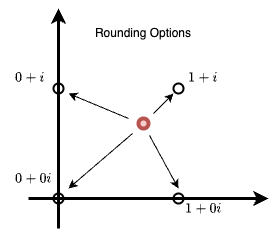
\includegraphics[width=0.4\textwidth]{Figures/RoundingOptions.png}
        \end{center}
        \begin{minipage}[t]{0.4\textwidth} % Adjust the width as needed
            \centering
            \vspace{0.1in}
            \begin{tabular}{c|c c}
                & $d(r) < d(div)$ \\ \hline
                1) & $13 < 82 \ \ $ &$\checkmark$ \\
                2) & $45 < 82 \ \ $ &$\checkmark$ \\
                3) & $53 < 82 \ \ $ &$\checkmark$ \\
                4) & $85 \not< 82 \ \ $ &$\times$ (NOT OK)
            \end{tabular}
        \end{minipage}%
        \hfill % Add space between the minipages
        \begin{minipage}[t]{0.55\textwidth} % Adjust the width as needed
            \begin{align}
                (6+7i) &= \overbrace{(9+i)}^{\text{divisor}}
                          \overbrace{(1+i)}^{\text{quotient}} + 
                          \overbrace{(-2-3i)}^{\text{remainder}} \nonumber \\
                       &= (9+i)(1+0i)+ (-3+6i) \nonumber \\
                       &= (9+i)(i) + (7-2i) \nonumber \\
                       &= (9+i)(0) + \underbrace{(6+7i)}_{36+49 \rightarrow 85} \nonumber 
            \end{align}
        \end{minipage}
        When uniqueness of $q,r$ is desirable, add this more stringent condition:
        \begin{enumerate}[i)]
            \item in $\Z$ require $0\leq r < |div|$
            \item in $\Z[i]$ use ``standard rounding'' ($\geq 0.5$ round up, $<0.5$ round down)
        \end{enumerate}
    \end{enumerate}
    \newpage
    So we have 
    \begin{center}
        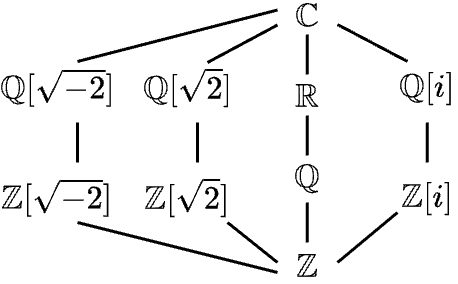
\includegraphics[width=0.5\textwidth]{Figures/ComplexRingLattice.png}
    \end{center}
    As an aside, when you see $\Z[\sqrt{integer}] = \{a+b\sqrt{int} \ | \ a,b \in \Z\}$ rings of this form are referred to as \textit{rings of quadratic integers} \index{Rings of Quadratic Integers}, they are quite important in Number Theory.
    Ok that concludes Example 3.9.6 :P
\end{example}
\begin{example}
    Any field is a Euclidean Ring. $\forall \ x \in F$ field, $x\neq 0$ define $d(x)=8 \ \ \leftarrow \text{ your favorite natural number}$
    \begin{enumerate}
        \item $d(x) \underset{\substack{\uparrow \\ \text{always equal}}}{\leq} d(xy)$
        \item $x=(xy^{-1})y +\underset{\substack{\uparrow \\ r}}{0} \ \ \ \text{ in }F, \ \ x\div y \text{ is }xy^{-1}$
    \end{enumerate}
\end{example}
\noindent We can now update our little diagram on Ring Classifications
\begin{figure}[h!]
    \centering
    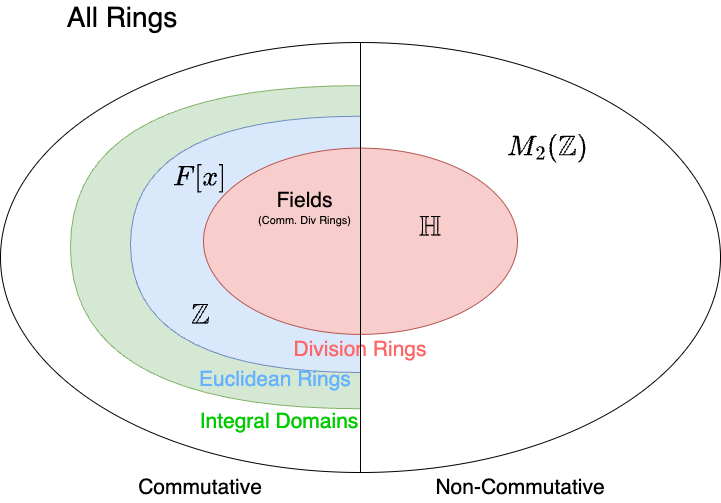
\includegraphics[width=0.9\textwidth]{Figures/RingClassifications_Euclidean.png}
    \caption{Ring Classifications (Updated)}
    \label{fig:ring-classifications-eucl}
\end{figure}
\begin{tcolorbox}
    \begin{center}
        Exam III Material Ends Here
    \end{center}
\end{tcolorbox}
\begin{tcolorbox}
    We briefly jumped ahead to some section 3.9 material from Herstein's book, we will now return to 3.7 material, I hope this wasn't too confusing...
\end{tcolorbox}
\newpage

\setcounter{section}{6}
\section{Principal Ideal Domains (3.7 Continued, sorry for the jump!)}
We know we can take $a\in R$ and generate $Ra$. But if we have an arbitrary ideal $U$ in $R$, you might or might not have a (single) generator. 
When an ideal can be generated in such a way (from a single element) we give it a special name, and when every ideal in a given ring has this property that ring gets a special name.
\begin{definition}[Principal Ideals and Principal Ideal Domains]
    Given $R$ integral domain.
    \begin{enumerate}
        \item An ideal $U$ in $R$ is \textit{principal} if it can be generated by a single element in $U$
        \begin{align}
            U \text{ principal }\iff \exists a \in U \ni U = Ra \nonumber
        \end{align}
        \item $R$ is a \textit{principal ideal domain} (PID) if every ideal in $R$ is principal.
    \end{enumerate}
\end{definition}
$\Z$ is a principal ideal domain (PID) since each of the ideals in $\Z$ take the form $n\Z$ ($n$ is the generator). 
\begin{theorem}
    If $R$ is a Euclidean ring, then $R$ is a PID.
    \begin{align}
        \boxed{\text{ Euclidean }\implies \text{ PID }}\nonumber
    \end{align}
    \textit{Proof:} Suppose $R$ is a Euclidean ring. \\ \steezybreak
    \noindent Easy case first: 
    \begin{align}
        \underbrace{\{0\}}_{\substack{\uparrow \\  \text{ideal}}} = R\cdot \underbrace{0}_{\substack{\uparrow \\ \text{generator}}} \ \ \ \therefore \ \ \ \{0\} \text{ is principal}. \nonumber
    \end{align}
    Take $U$ ideal in $R$, $U\neq \{0\}$ \\ 
    \noindent $R$ Euclidean $\implies \ \forall$ non-zero $a\in R \ \exists $ non-negative integer $d(a)$ (the ``size'' of $a$) \\
    \noindent Choose $x$ non-zero in $U$ with $d(x)$ minimal among all elements of $U$. \\
    \noindent \textbf{Claim:} $x$ generates $U$ (i.e. $U=Rx$) \\
    \noindent \textbf{$\supseteq$:} $\forall \ r \in R$, $rx\in U$ (since $r\in R$, $x\in U$ and $U$ ideal) so $Rx\subseteq U$ \\
    \noindent \textbf{$\subseteq$:} Take $y\in U$ \\
    \noindent $R$ Euclidean $\implies \ \exists \ q,r \in R \ni \ y=qx+r$ where $r=0$ or $d(r)<d(x)$ \\
    
    \begin{align}
        y\in U, \ \ qx &\in U \ \ &\text{ by absorp. } (q\in R, x\in U) \nonumber \\
        -(qx) &\in U \ \ \ &\text{ by }+ \text{ inv. }(U<R) \nonumber \\
        \therefore \ y+(-(qx)) &\in U, \ &\text{ so }r=y-qx \in U \nonumber
    \end{align}
    Since $d(r)<d(x)$ contradicts our choice of $x$ with minimal $d$-value, it must be true that $r=0$ \\
    \noindent $\therefore \ \ y=qx \in Rx$ \\
    \noindent $\therefore \ \ U\subseteq Rx$. $\blacksquare$
\end{theorem}

\begin{definition}[Divides (relation on comm. ring $R$)]
    Given $R$ commutative ring and $a,b\in R, \ a\neq 0$ the \textit{divides} relation is defined as follows
    \begin{align}
        a |b \iff \ \exists \ c\in R \ni \ b=ca \nonumber
    \end{align}
    That is, $a$ divides $b$ if and only if there exists some $c\in R$ for which $b=ca$
\end{definition}
\newpage
\begin{definition}[Greatest Common Divisor (for general comm. ring $R$)]
     Given $R$ commutative ring and $a,b, d \in R, \ d\neq 0$ $d$ is \textit{a greatest common divisor of $a$ and $b$} if and only if 
     \begin{enumerate}
        \item $d|a$ and $d|b$
        \item if $c$ is another common divisor then $c|a$ and $c|b$ $\implies \ c|d$.
     \end{enumerate}
\end{definition}

\begin{lemma}
    Let $R$ Euclidean ring. Any two non-zero elements $a,b \in R$ have a GCD. Moreover, $\exists \ \lambda, \mu \in R \ni$
    \begin{align}
        GCD(a,b) &= \lambda a + \mu b \nonumber
    \end{align}
    \textit{Proof:} Consider $U=\{ra+sb \ | \ r,s \in R \}$, $U$ is an ideal because it is $Ra+Rb$ \\ \steezybreak
    Now, $R\ \text{Euc.} \implies R \ \text{PID} \implies U=Rd$ for $d\in U$ \\ \steezybreak
    $d\in U \implies \ \exists \ \lambda, \mu \in R \ni \ d=\lambda a + \mu b$ \\ \steezybreak
    It remains to show that $d$ satisfies the definition of a GCD: \\
    \begin{enumerate}[(i)]
        \item $a=1\cdot a + 0\cdot b\in U = Rd$\\
        so $\exists \ r\in R \ni a=rd \ \therefore \ d|a$ \\
        $b=0\cdot a + 1\cdot b \in U = Rd$ \\
        so $\exists \ s\in R \ni b=sd \ \therefore \ d|b$ \\
        \item Suppose $c|a$ and $c|b$  $\implies \ \exists \ r,s \in R \ni a=rc  \text{ and } b=sc$ \\
        So
        \begin{align}
            d &=\lambda a + \mu b \nonumber \\
            &= \lambda (rc) + \mu (sc) \nonumber \\
            &= c \underbrace{(\lambda(r) + \mu (s))}_{\in R} \nonumber \\
            &\therefore \ c|d. \ \ \ \ \blacksquare \nonumber
        \end{align} 
        
    \end{enumerate}
\end{lemma}
\begin{example}[Application of Lemma 3.7.1 ]
\textbf{Application in $\R[x]$:} \\
If $GCD(f(x),f'(x))$ is constant, then $f(x)$ has no multiple roots. \\ \steezybreak
\textit{Proof:} (by contradiction)
Suppose $r$ is at least a double root of $f(x)$, then
\begin{align}
    f(x)&= (x-r)(x-r)g(x) \nonumber \\
    &= (x-r)^2 g(x) \nonumber
\end{align}
So $x-r|f(x)$
\begin{align}
    f'(x)&=2(x-r)g(x)+(x-r)^2 g'(x) \nonumber \\
    &= (x-r)[2g(x)+(x-r)g'(x)] \nonumber
\end{align}
So $x-r|f'(x)$ \\
$ \therefore \ x-r| GCD(f(x),f'(x)), $ \\
$GCD(f(x),f'(x))\text{ is constant by hypothesis, say it's }s\in \R$
\begin{align}
    \underset{\substack{\uparrow \\ \deg=0}}{s}&= \underbrace{(x-r)\cdot P(x)}_{\substack{\in \R[x] \\ \deg(x-r)+\deg(P(x))}} \ \ \ \ (P(x)\neq 0, \text{ otherwise } s=0) \nonumber
\end{align}
So $0= 1+ \underbrace{\deg(P(x))}_{\geq 0} \geq 1 \ \ \ \ \Rightarrow \Leftarrow$ \\
$\therefore$ there is no double root or larger for $f(x). \ \ \ \blacksquare$

\end{example}

After having seen several results, that were originally introduced for integers, generalized to arbitrary commutative rings, one might start to wonder about other properties that $\Z$ has and whether they too can be generalized.
For example, we know that element in $\Z$ have unique prime factorizations, for example
\begin{align}
    20&= 2^2\cdot 5 \nonumber
\end{align}
can we generalize the notion of ``prime''? We will get to this but it will take a little work, to start we present this definition
\begin{definition}[Unit (of a Commutative Ring)]
    Let $R$ be a commutative ring. $a\in R$ is a \textit{unit} if $\underset{\substack{\uparrow \ \ \ \ \ \  \ \\ mult. inv.}}{a^{-1}\in R}$ \\ \steezybreak
    $R^*$ denotes the set of units in $R$.
\end{definition}

\begin{proposition}[Units Fact \#1]
    $R^*$ is a group under $\cdot$ in $R$. \\

    \noindent \textit{Proof:} \\
    \indent $1\in R^*$  ($1=1^{-1}$) shows that $R^* \neq \emptyset$, in this group $1$ acts as $e$ (identity) under $\cdot$
    \begin{itemize}
        \item \textbf{Closure:} $r,s \in R \ \implies \ \exists \ r^{-1},s^{-1} \in R$, 
        \begin{align}
            (rs)(s^{-1}r^{-1})&= rer^{-1}=e \in R^* \nonumber
        \end{align}
        so $(rs)$ also has an inverse in $R$ (namely $s^{-1}r^{-1}$) and so $R^*$ is closed under $\cdot$
        \item \textbf{Associativity:} Inherited from $R$.
        \item \textbf{Identity:} $1\in R$
        \item \textbf{Inverses:} $r\in R^* \ \implies \ r^{-1} \in R \text{ and } (r^{-1})^{-1}=r\in R$ therefore $r^{-1}\in R^*. \ \ \ \ \blacksquare$
    \end{itemize}
\end{proposition}

\begin{example}[The units in the integers]
    $\Z^{*}= \{-1,1\}$ \\ \steezybreak
    
    \begin{tabular}{|c|c|c|}
        *&1&-1 \\ \hline
        1&1&-1 \\ \hline
        -1&-1&1 
    \end{tabular}
\end{example}
\begin{example} [The units of a field]
    Given $F$ field, $F^*=F-\{0\}$
\end{example}

\begin{example}[The units of polynomials over a field]
    $F$ field. $F[x]^* = \{\text{ constant polynomials }\} = F-\{0\}=F^*$ \\ \steezybreak
    \noindent Note if $f$ has inverse $g$, then $\underset{\substack{\ \\ \nwarrow \ \ \ \ \ \ \ \nearrow \\ non-zero}}{f(x)\cdot g(x)}=1$ \\ 
    \noindent and we get $\deg(fg)=\deg(f)+\deg(g)=0 \ \implies \deg(f)=\deg(g)=0$ \\
\noindent $\therefore \ f(x)=a_0 \neq 0$ and $g(x)=b_0 \neq 0$ \\
\end{example}
\newpage
\begin{proposition}[Units fact \#2]
    \begin{align}
        x\in \Z_n^* \iff \ x \text{ and } n \text{ are relatively prime in }\Z. \nonumber 
    \end{align}
    \textit{Proof:}\\
    \noindent $\Rightarrow :$
    \begin{align*}
        &x \in \Z_n^* \implies \exists \ y \in \Z_n \; \text{such that} \; xy =1 \text{ in }\Z_n \\
        &\text{So in } \Z, \; \exists \ k \in \Z \; \text{such that} \; xy = 1 + kn \\
        &\implies xy + (-k)n = 1 \\
        &\text{Since } GCD(x, n) \mid n \; \text{and} \; GCD(x, n) \mid x \implies GCD(x, n) \mid \underbrace{\big(xy + (-k)n\big)}_{1} \\
        &\implies GCD(x, n) = 1
    \end{align*}
    $\Leftarrow :$
    \begin{align*}
        &GCD(x, n) = 1 \\
        &\implies \exists \ s, t \in \Z \ni \; sx + tn = 1 \quad \text{( Lemma 1.3.1 )} \\
        &\implies n \mid (1 - sx) \\
        &\implies 1 \equiv sx \mod n \\
        &\text{Reduce } s \mod n: \; s \equiv \bar{s} \mod n, \; \text{where } \bar{s} \text{ is between } 0 \text{ and } n
    \end{align*}
    \begin{align*}
        &0 \leq \bar{s} \leq n \\
        &s \equiv \bar{s} \mod n, \; x \equiv x \mod n \\
        &\implies sx \equiv \bar{s}x \mod n  \\
        &\implies 1\equiv \bar{s}x \mod n \quad \text{(transitivity of congruence)} \\
        &\text{So in } \Z_n, \; 1 = \bar{s}x \ \ \ (\bar{s}=x^{-1} \text{ in }\Z_n) . \ \ \ \blacksquare
    \end{align*}
\end{proposition}
\setcounter{dummy_lemma}{0}
\begin{corollary}[Corollary to Units Fact \#2]
    \begin{align*}
        o(\Z_n^*) &= \text{ \# of positive integers less than }n\text{ and relatively prime to n}\\
        &= \phi(n) \ \ \ \ (\text{Euler totient function})
    \end{align*}
    \textit{Proof:} follows directly from Units Fact \#2.
\end{corollary}
Recall in $\Z$, $n|m$ and $m|n \ \implies n=\underset{\substack{\uparrow \\ \Z^*=\{1,-1\}}}{\pm} m$
\setcounter{dummy_lemma}{1}
\begin{lemma}
    Let $R$ integral domain, $a,b$ both non-zero in $R$. \\
    \noindent If $a|b$ and $b|a$ then $a=ub$ where $u\in R^*$ \\
    \noindent \textit{Proof:} \\
    \noindent $b|a \ \implies \exists \ u \in R \ni \ a=ub$ (must show $\exists u^{-1} \in R$).
    \noindent $a|b \ \implies \exists \ x \in R \ni \ b=xa$
    \begin{align*}
        a&= ub =uxa=(ux)a
    \end{align*}
    Now, $R$ integral domain $\implies$ we can cancel non-zero $a$ \\
    \noindent $\implies 1=u\underset{\substack{\uparrow \\ u^{-1}}}{x} \ \implies u \in R^*$. $\ \blacksquare$
\end{lemma}

\begin{definition}[Associates]
    $R$ commutative ring. $a,b\in R$ are \textit{associates} if one is a unit times the other:
    \begin{align*}
        \underbrace{a=ub}_{u^{-1}a=b} \text{ for some } u\in R^*
    \end{align*}
\end{definition}

\begin{example}
    $R=\Z$, $R^*=\{1,-1\}$
    \begin{align*}
        \forall \ n \in \Z, \text{ associates of }n \text{ are }n,-n.
    \end{align*}
\end{example}

\begin{example}
    $R=\Z_8$, 
    \begin{align*}
        \Z_8^* &= \{\text{positive integers }<8 \text{ and relatively prime to }8\} \\
        &=\underbrace{\{1,3,5,7\}}_{\substack{ \text{group in }\Z_8 \\ \text{ under }\cdot \mod 8}}
    \end{align*}
    For example the associates of $2$ are $\{2,6\}$
    \begin{align*}
        2\cdot 1 &= 2 \\
        2\cdot 3 &= 6 \\
        2\cdot 5 &= 2 \\
        2\cdot 7 &= 6 
    \end{align*}
\end{example}
\begin{tcolorbox}
    \textbf{Aside about Euclidean Rings:} \\ \steezybreak
    $R$ Euclidean $\implies$ $R$ PID \\
    $R$ Euclidean $\implies$ $\exists \ d: R-\{0\}\rightarrow \N \ni d(a)\leq d(ab) \ \forall \ a,b\in R-\{0\}$ \\
    $R$ Euclidean with non-zero $U$ (ideal), $U$ has the form $\underset{\substack{\ \ \  \uparrow \\ \text{generator }\neq 0}}{Rx}$ and $d(x)\leq \underset{\substack{\uparrow \\ \neq 0}}{d(rx)}$\\
    So generator has smallest possible size among non-zero elements in $U$. \\
    Also, in the proof of Theorem 3.7.1 we showed any non-zero element of smallest size is capable of generating $U$.
\end{tcolorbox}

\begin{lemma}
    Let $R$ Euclidean, $a,b$ non-zero in $R$. \\
    \noindent If $b\not\in R^*$, then $d(a) \underset{\substack{\uparrow \\ \text{strict}}}{<}d(ab)$ \\ \steezybreak
    
    \noindent \textit{Proof:} Assume $b\not\in R^*$ \\
    $R$ Euclidean $\implies \ d(a)\leq d(ab)$ \\
    Now assume $d(a)=d(ab)$ (we will try to arrive at a contradiction) \\
    Use $a$ to generate ideal $U=Ra$, by the aside above, $a$ must have smallest size possible among non-zero elements of $U$ \\
    $ab\in U$ by absorption ($a\in U$, $b\in R$), now since $d(a)=d(ab)$ that means $ab$ is also capable of generating $U$, so $U=R(ab)$, then $\exists \ r\in R \ni a=r(ab)=(rb)a$. \\
    $R$ Euclidean $\implies$ $R$ integral domain $\implies$ we can cancel non-zero $a$ \\
    $1=rb$ $\implies \ b\in R^* \ \ \Rightarrow \Leftarrow$ \\
    $\therefore \ d(a)\neq d(ab)$ \\
    $\therefore \ d(a)<d(ab). \ \ \blacksquare$ 
\end{lemma}
\setcounter{dummy_lemma}{2}
\begin{corollary}
    All units have the same size, namely $d(1)$, and $d(\text{unit})<d(\text{non-unit})$ \\ \steezybreak

    \textit{Proof: }
    Take $u\in R^*$, $\exists \ u^{-1}$ (non-zero) \\
    \begin{align*}
        d(u)&\leq d(uu^{-1})=d(1)\\
        d(1)&\leq d(1\cdot u) = d(u)
    \end{align*}
    
    $\implies \ d(u)=d(1)$ \\ \steezybreak

    Take $x\in R \ni x\not \in R^*$
    \begin{align*}
        d(u)&=d(1) \underset{L \ 3.7.3}{<}d(1\cdot x) = d(x). \ \ \ \blacksquare
    \end{align*}
\end{corollary}

\begin{definition}[Prime]
    \label{def:prime}
    $R$ Euclidean ring, $\pi \in R, \pi \neq 0$. \\ \steezybreak

    $\pi$ is \textit{prime} if whenever $\pi=ab$ for $ab\in R$, 
    \begin{align*}
        \text{Either } &a\in R^* \text{ and } b \not\in R^*, \\
        \text{or } &a\not\in R^* \text{ and } b\in R^*
    \end{align*}
    In other words, $\pi$ is prime if the only way it factors is as a unit times a non-unit
\end{definition}

\begin{tcolorbox}
    \textbf{Observation:} Consider $x$ both \textit{prime} and \textit{unit}. 
    \begin{align*}
        \underset{\substack{\uparrow \\ \text{prime}}}{x}&= \underset{\substack{\uparrow \\ \text{unit}}}{1}\cdot \underset{\substack{\uparrow \\ \text{non-unit}}}{x} \ \ \ \Rightarrow \Leftarrow \\
        \implies &\{\text{primes}\}\cap \{\text{units}\} = \emptyset
    \end{align*}
    \begin{center}
        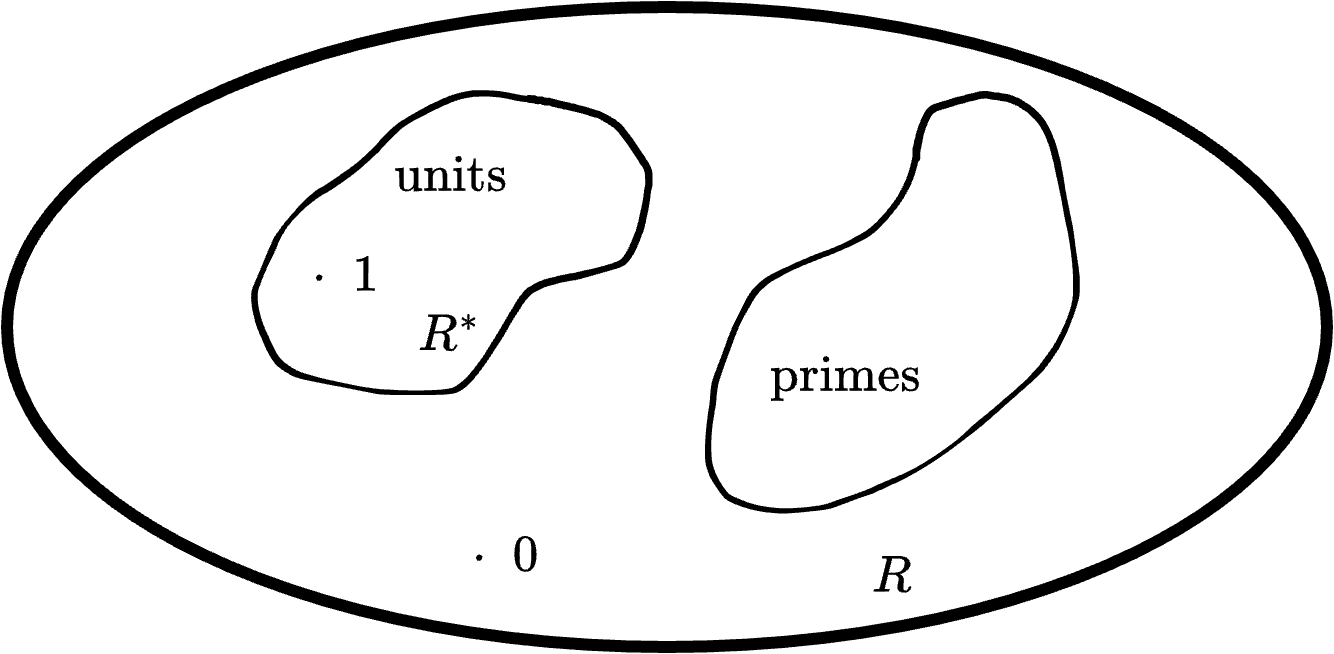
\includegraphics[width=0.5\textwidth]{Figures/UnitsAndPrimesAreDistinct.png}
    \end{center}
\end{tcolorbox}
\newpage 
\section*{Things to know for Exam III}
\subsection*{Rings}
You should know the basic properties of rings, as well as the different types of rings we discussed and the properties that make them distinct from others:

You should be familiar with:
\begin{itemize}
    \item \textit{Integral Domains} 
    \item \textit{Fields}
    \item \textit{Division Rings}
    \item \textit{Euclidean Rings} (these have a size function)
\end{itemize}
You should also be familiar with:
\begin{itemize}
    \item\textit{Subrings}
    \item \textit{Ideals} ($U_1\cap U_2, \ U_1+U_2, \ Rx$)
    \item \textit{Center}
    \item \textit{Annihilator of an Ideal}
    \item \textit{Centralizer of an Element}
    \item \textit{Direct Product of Rings}
\end{itemize}
As well as
\begin{itemize}
    \item \textit{Zero divisors}
    \item \textit{Idempotent} (HW \#11)
    \item \textit{Ring homomorphisms}
    \item \textit{Kernels}
\end{itemize}
\subsection*{The ring of Integers $\Z$}
Should be familiar with 
\begin{itemize}
    \item Ideals in $\Z$ ($n\Z$s)
    \item $n\Z\cap m\Z$
    \item $n\Z+m\Z$
    \item $n\Z \text{ maximal }\iff n \text{ is prime.}$
\end{itemize}
\subsection*{Division in Various Rings}
You should be familiar with division in:
\begin{itemize}
    \item $\H$
    \item $\C$
    \item $\Z[i]$
    \item $\R$
    \item $\Z_p$
    \item $\Q$
    \item $F[x]$
    \item $\Z$
\end{itemize}
\subsection*{Theorems}
You should be familiar with the following theorems and major results
\begin{itemize}
    \item Structure Theorem for Finite Abelian Groups
    \item First Isomorphism Theorem for Rings
    \item $R/U \text{ field } \iff \ U \text{ maximal}$
    \item Any integral domain $D$ (e.g. $\Z$) can be extended to a field $F$ (e.g. $\Q$) (Know proof construction)
\end{itemize}
\newpage 

Recall from definition \ref{def:prime} that non-zero $\pi \ \text{ prime }\iff \ \pi \text{ factors only as }(\text{unit})(\text{non-unit})$\\
$\implies \{\text{prime}\}\cap R^*=\emptyset$\\ \steezybreak

Furthermore, Lemma 3.7.3 tells us that given $a,b\in R-\{0\}$, $b\not\in R^* \ \implies \ d(a)<d(ab)$
\section*{Factorization in $R$ Euclidean}
\begin{lemma*}[Factorization Lemma \#1]
    \index{Factorization Lemma \#1}
    Given $a,b\in R-\{0\}$, $R$ Euclidean
    \begin{align*}
        b\not\in R^* \implies Rab \varsubsetneq Ra
    \end{align*}
    \textit{Proof:} \\ \steezybreak
    Take $r\in R$, then $rab = \underbrace{(rb)}_{\in R}a \in Ra$, so $Rab\subseteq Ra$. \\

    \noindent Now assume $Rab=Ra$ (try for a contradiction) \\
    $a\in Ra$ as $1\cdot a$ so $\exists \ r \in R \ni a=rab$
    \begin{align*}
        R \text{ Eucl. } &\implies R \text{ integral domain } \implies \ \text{ cancellation holds } \\
        &\implies \ 1=rb \ \implies \exists \ b^{-1}\in R \ \implies \ b\in R^* \Rightarrow \Leftarrow \ b\not \in R^* \\
        &\therefore \ Rab \varsubsetneq Ra. \ \ \ \blacksquare
    \end{align*}
\end{lemma*}
\begin{example}
    In $\Z$, taking $a=2$ and $b\underset{\substack{\uparrow \\ \text{non-unit}}}{=2}$, $\ Ra=2\Z$, $Rab=4\Z$, $4\Z \varsubsetneq 2\Z$
\end{example}

\begin{lemma*}[Factorization Lemma \#2]
    \index{Factorization Lemma \#2}
    If $U_1 \subseteq U_2 \subseteq U_3 \cdots$ are ideals of commutative ring $R$, then 
    \begin{align*}
        U &= \bigcup_{i=1}^\infty U_i \text{   is an ideal of }R
    \end{align*}
    \textit{Proof:} $U\neq \emptyset$ since $0\in U_1$ so $0\in U$, so Lemma 2.4.1 applies. Take $x,y\in U$, then $x\in U_i$ for some $i$ and $y\in U_j$ for some $j$
    \begin{align*}
        \text{Nesting } \implies \ x,y \text{ are both in } U_{\max(i,j)},
    \end{align*}
    $U_{\max(i,j)}$ is an ideal so it is closed under $+$
    \begin{align*}        
        \therefore \ x+y \in U_{\max(i,j)} \subseteq U.
    \end{align*}
    So $U$ has $+$ closure. \\
    \textbf{Absorption:} Take $r\in R$, $x$ as above
    \begin{align*}
        U_i \text{ ideal }& \implies \ rx \in U_i \text{ by absorption in }U_i \\
        \text{ and }U_i \subseteq U &\implies \ rx \in U 
    \end{align*}
    \begin{tcolorbox}
        Note that additive inverses follow from absorption:
        \begin{align*}
            -x &= \underbrace{(-1)}_{\in R}\underbrace{x}_{\in U_i} \in U_i \ \text{ by absorption}. 
        \end{align*}
        This is a useful shortcut for showing $+$ inverses.
    \end{tcolorbox}
    $\therefore \ U \text{ is and ideal}. \ \ \blacksquare$
\end{lemma*}

\begin{lemma}[Factorization Theorem]
$R$ Euclidean $r\in R-\{0\}$ and $r\not\in R^*$, then $r$ is a product of finitely many primes\footnote{This lemma is important enough to consider it a theorem, but we continue with the naming used by Herstein}. \\ \steezybreak
\begin{center}
    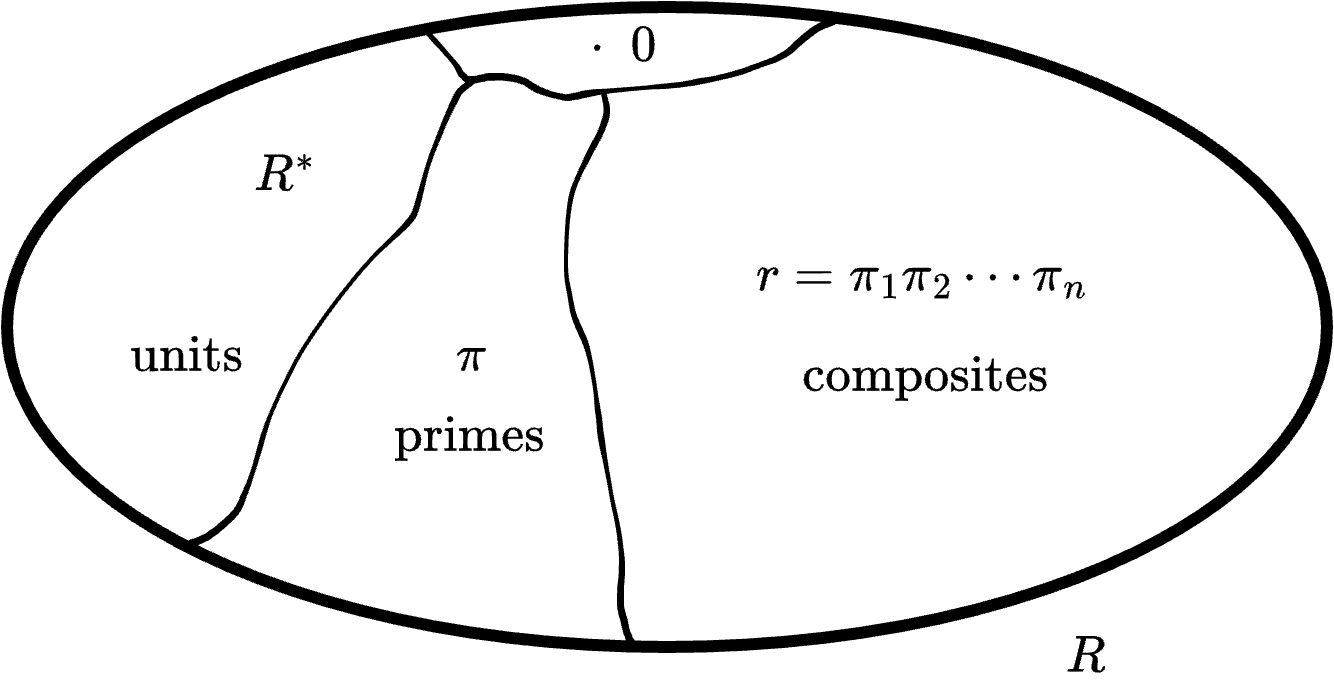
\includegraphics[width=0.65\textwidth]{Figures/UnitsPrimesComposites.png}
\end{center}
\textit{Proof: } \\ \steezybreak

Let $S= \{0\} \cup R^* \cup \{\text{primes}\}\cup \{\text{composites}\}$ (we will show $R-S=\emptyset$)\\ \steezybreak

\noindent Suppose $\exists \ x\in R-S$, $x$ isn't prime so it has a factorization other than $(\text{unit})(\text{non-unit})$ (both units or both non-units)
If $x=ab, a,b \in R^*$ then since $R^*$ group ($\cdot$ closure) $\implies$ $x\in R^* \ \Rightarrow \Leftarrow \ \because x \not\in S$\\ \steezybreak

\noindent So it must be that $x=ab, a,b \not\in R^*$ (neither $a$ nor $b$ is a unit). \\
We also note $a,b$ are not $0$ otherwise $x=0$ ($\Rightarrow \Leftarrow \ x\not\in S$). \\ \steezybreak

Consider where the factors lie
\begin{align*}
    &\text{If }a\in S, \text{ then }a \not \in R^* \ \text{ and }a\neq 0 \\
    &\implies \ a \text{ is the product of finitely many primes}
\end{align*}
The same argument would apply to $b$. But if $a,b \in S$ and are products of finitely many primes then $x=ab$ is also a product of finitely many primes! $\Rightarrow \Leftarrow \ \because x\not\in S$. \\

So $a\in R-S$ or $b\in R-S$ (or both). Without loss of generality (WLOG) say $a\in R-S$
\begin{align*}
    \text{Factorization Lemma \#1} \implies \text{ Since }a\neq 0 \text{ and }b \text{ non-unit}\\
    R\underbrace{ab}_{x}\varsubsetneq Ra
\end{align*} 
\begin{align*}
    a\in R-S &\implies \ a=cd \text{ where }c\in R-S \ (\text{ so }c\neq 0) \text{ and }d\in R^* \\
    &\implies Rx \varsubsetneq Ra \varsubsetneq Rc \varsubsetneq \cdots \text{ keep iterating to build ascending chain of ideals} \\
    &\ \ \ \ \ \ \ \ \ \ U_1 \varsubsetneq U_2 \varsubsetneq U_3 \varsubsetneq \cdots \text{ Rename and call union of this nested chain }U \\
    \text{Factorization Lemma \#2 }&\implies \ U \text{ is an ideal} \\
    R \text{ Euclidean }\implies \ R \text{ PID } &\implies \exists \ g\in R \ni U=Rg \ (\text{ single generator })\\
    g\in U &= \bigcup_{i=1}^\infty U_i \implies \exists \ j \in \Z \ni \ g\in U_j  \\
    R\underset{\substack{\uparrow \\ \in U_j}}{g} &\subseteq U_j \varsubsetneq U_{j+1} \varsubsetneq U = Rg \\
    &\Rightarrow \Leftarrow \ Rg \text{ can't be smaller than itself} \\
    &\therefore R-S=\emptyset \\
    &\therefore R=S. \ \ \ \blacksquare 
\end{align*} \footnote{Note, in the fourth to last line, there will always be a $U_{j+1}$ because if there weren't $x$ would admit a finite composite representation $\Rightarrow \Leftarrow$ }
\end{lemma}

Whats left to do: Questions of uniqueness (both of GCDs and the Factorization just covered). Also what does a notion of relatively prime look like here?

\begin{theorem*}[GCD Relationship Theorem]
    \index{GCD Relationship Theorem}
    $R$ Euclidean, $a,b \in R-\{0\}$, with $GCD(a,b)=d$
    \begin{align*}
        d' =GCD(a,b) \iff d \text{ and }d' \text{ are associates in }R
    \end{align*}
    \textit{Proof:} \\ \steezybreak
    $\Rightarrow:$ Assume $d$ and $d'$ are both GCDs of $a$ and $b$, then 
    \begin{align*}
        \underset{\substack{\text{common}\\ \text{divisor}}}{d}|\underset{\text{GCD}}{d'} \text{  and  } \underset{\substack{\text{common}\\ \text{divisor}}}{d'}|\underset{\text{GCD}}{d} \overset{L3.7.2}{\implies} \ \exists \ u \in R^* \ni \ d'=ud \ (d'\text{ and }d\text{ are associates.})
    \end{align*}
    $\Leftarrow:$ Take any $u\in R^*$ to form arbitrary associate 
    \begin{align*}
        ud=d' \ \ \ (\text{ we will show }d' \text{ satisfies the definition of GCD.})
    \end{align*}
    \begin{align*}
        \text{Hypothesis }&\implies d|a \ \implies \exists \ x\in R \ni a= dx \\
        u \in R^* &\implies \exists \ u^{-1}\in R \ (\text{ actually it's in }R^*)\\
        &\text{So } a=d(uu^{-1}x) = \underbrace{(du)}_{d'}\underbrace{(u^{-1}x)}_{\in R} \implies \ d'|a
    \end{align*}
    Similarly $d|b \ \implies \ d'|b$\\
    Now suppose $c$ is a common divisor of $a,b$. Then $c|\underset{\substack{\uparrow \\ \text{GCD}}}{d}$ so $\exists \ r\in R \ni d=rc$, but then 
    \begin{align*}
        d'&=ud=u(rc) = \underbrace{(ur)}_{\in R}c \\
        &\implies \ c|d' \\
        &\therefore \ d' \text{ is a GCD of }a \text{ and }b. \ \ \ \blacksquare
    \end{align*}
\end{theorem*}
This theorem basically says that if we have one $GCD$ we've got them all by using $R^*$
\begin{align*}
    \{\text{GCDs of }a,\ b\} &= \{u\cdot \underbrace{GCD(a,b)}_{\substack{\uparrow \\ \text{one}\\ \text{we} \\ \text{have}}} \ | \ u \in R^*\}
\end{align*}
In a Euclidean ring $R$, GCDs are ``Unique up to associates''. 

\begin{example}
    In $\Z$ Euclidean, $\Z^*=\{1,-1\}$ 
    \begin{align*}
        \{\text{ GCDs of }9, \ 6\}&= \{-3,3\}
    \end{align*}
    Theorem guarantees that this is the complete set of GCDs of $9$ and $6$ \\ \steezybreak
    In simplified presentation of $\Z$ we define GCD as positive to cut it down to one GCD.
\end{example}

\begin{definition}[Relatively Prime]
    $R$ Euclidean, $a,b \in R-\{0\}$, $a$ and $b$ are \textit{relatively prime} iff $GCD(a,b)\in R^*$
\end{definition}
This well-defined because if one $GCD(a,b)$ is a unit, they all have to be:
\begin{align*}
    \{\text{ Complete set of GCDs of }a, \ b\}= \{\underset{\substack{\uparrow \\ \text{unit}}}{u}\cdot \underset{\substack{\uparrow \\ \text{unit}}}{GCD(a,b)} \ | \ u\in R^* \} \subseteq R^* \ \ (\text{ closed under }\cdot \ )
\end{align*}

\section*{Some Questions}
\begin{enumerate}
    \item \textbf{Q1:} What are the primes in $\Q$? 
    \item \textbf{Q2:} Are $9$ and $6$ relatively prime in $\Q$?
\end{enumerate}
\vspace{0.25in}
\begin{enumerate}
    \item \textbf{A1:} $\Q$ is a field so $\Q^*=\Q-\{0\}$, and since $\{\text{units}\}\cap \{\text{primes}\} =\emptyset$ $\implies \ \Q$ has no primes. \\
    Note, $0$ is neither prime nor a unit, but when $F$ is a field, $F^*$ is everything aside from $0$.
    \item \textbf{A2:} $GCD(9,6)=3$, now is $3$ a unit in $\Q$? Of course! $3,\ \frac{1}{3}=3^{-1}$ \\
    So $9$ and $6$ are relatively prime in $\Q$ (Actually everything is relatively prime in $\Q$)
\end{enumerate}
\vspace{0.2in}
\noindent Next on the agenda... Unique Factorization, do we get it in Euclidean $R$? We are almost ready to tackle that question but first, two more lemmas that generalize some results we encountered in chapter 1.
\begin{lemma}
    $R$ Euclidean, $a,b,c \in R$ $a,b \neq 0$.\\
If $a | bc$  and $a$ and $b$ are relatively prime, then $a|c$. \\

\noindent \textit{Proof: } $a$ and $b$ relatively prime $\implies \ GCD(a,b)=u \in R^*$ so $\exists \ \lambda, \mu \in R \ni u=\lambda a + \mu b$. Now multiply by $c$
\begin{align*}
    uc = \lambda \underset{\substack{\uparrow \\ a|a}}{ac} + \mu \underset{\substack{\uparrow \\ a|bc}}{bc}
\end{align*}
\begin{align*}
    a|a \text{ and }a|bc \implies a | \underbrace{(\lambda c)a+ (\mu)(bc)}_{uc}
\end{align*}
So $\exists \ r\in R \ni \ uc=ra$
\begin{align*}
    u \text{ unit } & \implies \exists \ u^{-1}\in R \text{ so left mult. by }u^{-1} \\
    & \ \ \ \ \ \ \ \ \ \ c=u^{-1}ra \\
    &\implies c= \underbrace{(u^{-1}r)}_{\in R} a \implies a|c.  \ \ \ \blacksquare 
\end{align*}
\end{lemma}

\begin{lemma}
    $R$ Euclidean with $a,b, \pi \in R, \ \pi \text{ prime}$.
    \begin{align*}
        \text{If }\pi | ab, \text{ then }\pi|a \text{ or }\pi|b
    \end{align*}
    \textit{Proof: } Trivial case first, if $ab=0$, then 
    \begin{align*}
        R \text{ Euclidean }&\implies \ R \text{ int. domain} \\
        &\implies \text{ either }a=0 \text{ or }b=0 \\
        0=0\cdot \pi \implies \ \pi | 0 \implies \ \pi | a \text{ or } \pi | b
    \end{align*}
    So now we may assume $ab\neq 0$, then neither $a$ nor $b$ is $0$ (Lemma 3.2.1 (i))\\
    Suppose $d$ is a $GCD(a,\pi)$
    \begin{align*}
        d|a &\implies \exists \ r\in R \ni a =rd \\
        d|\pi &\implies \exists \ s\in R \ni \pi = sd 
    \end{align*}
    \begin{align*}
        \pi \text{ prime }\implies \text{ either } &(i) \ d\in R^* \text{ and }s \text{ is not.} \\
        \text{ or }&(ii) \ s\in R^* \text{ and }d \text{ is not.} 
    \end{align*}
    If $(i)$, then $d\in R^* \ \implies a$ and $\pi$ are relatively prime, combining this with the hypothesis ($\pi|ab$) then by Lemma 3.7.5, $\pi|b$ \\

    \noindent If $(ii)$, then $s\in R^* \ \implies \exists \ s^{-1}\in R $
    \begin{align*}
        \pi &= sd \\
        \implies \pi s^{-1} &= d \\
        \text{ then }a&= rd =r\pi s^{-1}= \underbrace{(rs^{-1})}_{\in R}\pi \\
        &\therefore \ \pi | a. \ \ \ \blacksquare
    \end{align*}
\end{lemma}
\setcounter{dummy_lemma}{5}
\begin{corollary}
    Given $\pi$ prime in Euclidean ring $R$, then 
    \begin{align*}
        \pi | a_1 a_2 \cdots a_n \ \implies \ \pi | a_i \text{ for at least one } 1\leq i \leq n 
    \end{align*}
    \textit{Proof: } 
    \begin{align*}
        \pi | a_1 (a_2 \cdots a_n) \ &\implies \ \underbrace{\pi |a_1}_{\substack{\text{either we}\\ \text{found it}}} \text{ or  } \underbrace{\pi | a_2 \cdots a_n}_{\text{or not}}\\
        \text{ If not, }\pi | a_2 (a_3 \cdots a_n) &\implies \pi | a_2 \text{ or }\pi | a_3 \cdots a_n \\
        &\vdots \\
        &\implies \pi |a_{n-1}(a_{n-1}a_n) \implies \pi|a_{n-2} \text{ or }\pi | a_{n-1}a_n \\
        \text{ If not, } \pi |a_{n-1}a_n &\implies \pi | a_{n-1} \text{ or }\pi | a_n. \ \ \ \blacksquare 
    \end{align*}
\end{corollary}

In Euclidean $\Z$, primes are $\pm 2, \ \pm 3, \ \pm 5, \ \cdots $ and factorization is unique \textit{up to associates.}
\begin{align*}
    52&= \ \ \ \underset{\updownarrow}{2} \ \ \cdot \ \underset{\updownarrow}{2} \ \ \cdot \ \ \underset{\updownarrow}{13} \\
    &= (-2)\cdot 2 \cdot (-13) \\
    -13&= (-1)(13) \ \ \ \ \ \ \ \ \ \text{ so }-13 \text{ and }13 \text{ are associates.} \\
    2&=(1)(2), \ \ \ \ \ \ \ \ \ \ \ \ \ 2 \text{ is associate to itself}
\end{align*}
In any factorization of $52$ into primes, two will appear twice, bringing a unit ($1$ or $-1$), $13$ will appear once bringing at unit. \\ \steezybreak
\subsubsection*{The Unique Part:}
\begin{itemize}
    \item The positive primes involved.
    \item The number of appearances of each.
\end{itemize}
Note that since $\Z$ is commutative, the order in which the primes appear is irrelevant. In the simplified presentation of $\Z$ it is customary to add a condition that factoring be done in this way:
\begin{align*}
    \underbrace{(\pm 1)}_{\substack{\text{product}\\ \text{of} \\ \text{units}}}(\text{Product of positive primes listed smallest to largest})
\end{align*}
\begin{align*}
    \therefore \ \ \ 52&= (1)(2\cdot 2\cdot 13) = 2^2 \cdot 13 \\
    -52 &= (-1)(2\cdot 2\cdot 13 )= -(2^2\cdot 13)
\end{align*}
\setcounter{dummy}{1}
\begin{theorem}[Unique Factorization in $R$ Euclidean]
    Every non-zero element in Euclidean ring $R$ is either a unit or can be written uniquely up to associates as a product of finitely many prime elements of $R$. \\

    \noindent \textit{Proof: } Let $a$ be a non-zero non-unit in $R$,
    \begin{align*}
        \text{Factorization Theorem } \implies a=\pi_1 \pi_2 \cdots \pi_n, \ \ \pi_i \text{ prime}.
    \end{align*}
    Suppose $a$ also factors as $a= \tilde{\pi}_1 \tilde{\pi}_2 \cdots \tilde{\pi}_m,  \ \ \tilde{\pi}_j \text{ prime}$.
    \begin{align*}
        \pi_1| a &\implies \pi_1 | (\tilde{\pi}_1 \cdots \tilde{\pi}_m) \\
        &\underset{C3.7.6}{\implies} \pi_1 | \tilde{\pi}_j \ \text{ for some } 1\leq j \leq m \\
        &\implies \tilde{\pi}_j =u_1\pi_1 \text{ for some }u_1 \in R^* \ \ \ \ (\tilde{\pi}_j, \pi_1 \text{ prime, non-units means }u_1\text{ must be a unit})
    \end{align*}
    \begin{align*}
        \therefore \ \ \  \not \mathrel{\pi_1}\cdots \pi_n = \tilde{\pi}_1 \tilde{\pi}_2 \cdots \tilde{\pi}_{j-1} u_1 \not \mathrel{\pi_1} \tilde{\pi}_{j+1}\cdots \tilde{\pi}_m \ \ (\text{ can cancel }\pi_1 \text{ because }R\text{ integral domain.})
    \end{align*}
    Repeat process with $\pi_2$, $\pi_3$ etc. \\
    
    \noindent If $\pi$'s are exhausted first:
    \begin{align*}
        1=\underbrace{(u_1 u_2 \cdots u_n)\tilde{\pi}_{k_1}\cdots}_{\tilde{\pi}_{k_q}^{-1}?}\tilde{\pi}_{k_q} \implies \tilde{\pi}_{k_q} \text{ is a unit }\Rightarrow \Leftarrow
    \end{align*}

    \noindent If $\tilde{\pi}$'s are exhausted first:
    \begin{align*}
        \pi_{k_1}\cdots \pi_{k_q} &= \underbrace{(u_1\cdots u_m)}_{\substack{\text{unit }\\(\cdot \text{ closure in }R^*)}}\cdot 1 \\
        \implies 1=\underbrace{(u_1 u_2 \cdots u_m)^{-1}\pi_{k_1}\cdots}_{\pi_{k_q}^{-1}}\pi_{k_q}&= 1 \ \implies \pi_{k_q} \text{ is a unit }\Rightarrow\Leftarrow
    \end{align*}
    So they must be exhausted at the same time. \\

    \begin{align*}
        \text{ So, }a= \pi_1 \pi_2 \cdots \underset{n=m}{\pi_n} = (u_1\pi_1)(u_2 \pi_2)\cdots (u_n\pi_n)
    \end{align*}
    each factor in the $\sim$ factorization is associate to a factor in the original factorization. $\blacksquare$
\end{theorem}
\subsection*{Factorization In Polynomial Rings}
Given $F$ field, $F[x]$ is Euclidean with degree as ``size'' function.
\begin{lemma*}[Factors/Roots Connection]
    \index{Factors/Roots Connection (Polynomials Rings)}
    Suppose $f(x)\in F[x], \ a\in F$ then $f(a)=0 \iff (x-a)|f(x)$ in $F[x]$, i.e.
    \begin{center}
        \begin{align*}
            \boxed{ a \text{ is a root of }f \iff x-a \text{ is a factor of }f(x)}
        \end{align*}
    \end{center}
    \noindent \textit{Proof:} \\
    
    \noindent $\Leftarrow:$ Recall that the ``evaluation map'' is a ring homomorphism:
    \begin{align*}
        \phi_a: F[x]\rightarrow F \\
        \phi_a(f(x))=f(a)
    \end{align*}
    Now,
    \begin{align*}
        (x-a)|f(x) &\implies \exists \ g(x) \in F[x]\ni f(x)=g(x)(x-a). \\
        \text{ then }f(a) &= \phi_a(f(x))=\phi_a(g(x)(x-a)) \\
        &= \phi_a(g(x))\phi_a((x-a)) \\
        &= \underset{\in F}{g(a)}\underset{0\in F}{(a-a)} = g(a)\cdot 0 = 0. \\
        &\therefore \ \ a \text{ is a root of }f(x).
    \end{align*}
    \noindent $\Rightarrow :$ Assume $f(a)=0$. \\
    \begin{align*}
        F[x] \text{ Euclidean } &\implies \exists \ q(x), r(x) \in F[x] \ni f(x)=q(x)(x-a)+r(x) \\
        \text{ where either } &(i) \ r(x)=0  \\
        \text{ or } &(ii) \ \deg(r(x))< \underbrace{\deg(x-a)}_{1} 
    \end{align*}
    \begin{align*}
        \text{ if }&(ii) \deg(r(x))=0 \implies \ r(x)=a_0x^0 = a_0 \neq 0 
    \end{align*}
    \begin{align*}
        \text{ then } 0 = f(a) = \phi_a(f(x)) &= \phi_a(q(x))\phi_a(x-1)+\phi_a(r(x)) \\
        &= q(a)\cdot 0 + r(a) \\
        &= r(a)
    \end{align*}
    However $0=r(a)=a_0x^0 = a_0\cdot 1 = a_0$, but $a_0 \neq 0$! $\Rightarrow \Leftarrow, \ \ \therefore$ it must be $(i)$ \\
    $\implies \ (x-a)|f(x)$. $\blacksquare$
\end{lemma*}

\subsubsection*{Primes/Units in $F[x]$}
We saw earlier that $F[x]^*=F^* = F-\{0\}$, that is 
\begin{align*}
    \{\text{units in }F[x]\}= \{\text{deg }0 \text{ polynomials}\}.
\end{align*}
In $F[x]$ ``primes'' are known as \textit{Irreducibles}: they factor only as $\underset{\substack{\uparrow \\ coeff.}}{\text{unit}}\cdot\text{non-unit}$
\begin{align*}
    2x+4 &= 2(x+2)
\end{align*}
For example, $2x+3$ is irreducible in $\R[x]$
\begin{align*}
    2x+3 = 2\left(x+\frac{3}{2}\right)
\end{align*}
you might ask, couldn't we do something like:
\begin{align*}
    \underset{\substack{\\ \\ \ \ \nwarrow \ \ \ \ \ \ \ \ \ \ \ \ \ \ \nearrow \\ \text{ not in }R[x] \\ \sqrt{x}=x^{1/2} \text{ not even a polynomial}}}{(\sqrt{2x}+\sqrt{3})(\sqrt{2x}-\sqrt{3})} ?
\end{align*}
What the irreducibles are in $F[x]$ depends on $F$:\\
In $\C[x]: \\
f(x) \text{ is irreducible } \iff f(x) \text{ is linear } \ \ (\deg(f) =1)$. (``The Fundamental Theorem of Algebra'' [Gauss]) \\
Every $f(x) \in \C[x]$ is a product of \ul{linear} factors. That is, $\C$ is a \ul{splitting field}. \\
For example 
\begin{align*}
    f(x)=x^2+1 = (x+i)(x-i)
\end{align*}
In $\R[x]$: \\
$f(x)$ is irreducible
\begin{align*}
    x^2+1\in R[x] \\
    x= \frac{-b \pm \sqrt{\overbrace{b^2-4ac}^{<0}}}{2a}
\end{align*}
So in $\R[x]$ $f(x)$ is irreducible $\iff$ $f(x)$ is linear OR quadratic with negative discriminant ($b^2-4ac$)\\
\noindent In $\Q[x]$: \\
Spotty results (i.e. less general)
\newpage
\begin{tcolorbox}
    \index{Eisenstein Criteria for Irreducibility in $\Q[x]$}
    \textbf{Eisentein's Criteria:} \\ \steezybreak 
    If $f(x)=a_0+a_1x+ \dots + a_n x^n \in \Q[x]$ with $a_0, a_1, \dots, a_n \in \Z$ and if $\exists$ prime $p\in \Z\ni p \not | \ a_n$ but $p|a_i \ \ 0\leq i \leq n-1$ and $p^2 \not | \ a_0$ then $f(x)$ is irreducible in $\Q[x]$.
\end{tcolorbox}
\begin{example}
    Let $f(x)= x^4 + 10x + 5 \in \Q[x]$, note that the coefficients are in $\Z$ \\
    Now for $p=5$: $p|5$ and $p|10$ but $p\not | \ 1$ and $p^2 \not | \ 5$ \\
    $\therefore \ $Eisenstein says $f(x)=x^4+10x+5$ is irreducible in $\Q[x]$
\end{example}
\begin{lemma*}[Rational Root Test]
    \index{Rational Root Test}
    Suppose $f(x) = c_0 + c_1x + \dots + c_n x^n \in \Z[x] \subseteq \Q[x]$. \\
    If $\frac{a}{b} \in \Q$ is a root of $f(x)$ with $a$ and $b$ relatively prime (so $\frac{a}{b}$ is in ``lowest terms'' ) then $a|c_0$ and $b|c_n$. \\

    \noindent \textit{Proof: }
    \begin{align*}
        0 = f\left(\frac{a}{b}\right)= c_0 + c_1\left(\frac{a}{b}\right) + \dots + c_n\left(\frac{a}{b}\right)^n
    \end{align*}
    Clear the denominators
    \begin{align*}
        \underbrace{0\cdot b^n}_{0} =  c_0b^n + c_1ab^{n-1} + c_2a^2b^{n-2} + \dots + c_na^n
    \end{align*}
    Then
    \begin{align*}
        c_0b^n = -[c_1ab^{n-1} + \dots + c_na^n]
    \end{align*}
    Now, $a|RHS$ so $a|c_0b^n$, but $a$ and $b^n$ are relatively prime $\implies \ a|c_0$ \\
    Also,
    \begin{align*}
        c_na^n = -[c_0b^n + \dots + c_{n-1}a^{n-1}b]
    \end{align*}
    so $b| RHS$ which means $b|c_na^n$ and since $b$ and $a^n$ relatively prime $\implies \ \ b|c_n. \ \ \ \blacksquare$
\end{lemma*}
To find the roots of $p(x) \in \Z[x]$ look among the $\frac{a}{b}$'s where $a|c_0$ and $b|(\text{leading coefficient})$
\begin{example}
    Let $p(x)=3x^6+90x^5+\frac{161}{3}x^4-28x^3+21x-7\in \Q[x]$
    \begin{align*}
        3p(x)=9x^6+270x^5+161x^4-84x^3+63x-21
    \end{align*}
    Now note that $p(a)=0 \iff 3p(a)=0$ (i.e. they have the same roots)
    \begin{align*}
            &\Rightarrow: \text{ obviously }\\
            &\Leftarrow: \text{ integral domain }\therefore \ 3\neq 0 \implies p(a)=0
    \end{align*}
    Now lets look at the candidates for $\frac{a}{b}$
    \begin{align*}
        a|21 \implies a&= (\pm)1, \ 3, \ 7, \ 21 \\
        b|9 \implies b &= (\pm)1, \ 3, \ 9 \\
        \text{ So } \frac{a}{b} &= (\pm) \frac{1}{1}, \ \frac{1}{3}, \ \frac{1}{9}, \ \frac{3}{1}, \ \cancel{\frac{3}{3}}, \ \cancel{\frac{3}{9}}, \ \frac{7}{1}, \ \frac{7}{3}, \ \frac{7}{9}, \ \frac{21}{1}, \ \cancel{\frac{21}{3}}, \ \cancel{\frac{21}{9}} \ (\text{keep lowest terms versions})
    \end{align*}
    Let's start plugging them in and see if we can find a root/factor.
    \begin{align*}
        p(1)&= 79+ \frac{161}{3} \neq 0 \\
        p(-1)&= -87 + \frac{161}{3} \neq 0 \\
        p\left(\frac{1}{3}\right) &= 0 \ \implies \ \left(x- \frac{1}{3}\right) \text{ is a factor of }p(x)
    \end{align*}

    \begin{align*}
        (x-\frac{1}{3}) \ \ &\stackon[1pt]{\showdiv{ \ \ p(x) \ \ \ \ }}{ \ \ q(x) \ \ \ \ } \\
        \implies p(x)&=\left(x-\frac{1}{3}\right)q(x) \\
        q(x)&=(3x^5+91x^4+84x^3+21) \ \ \ \ \text{ integer coefficients so check Eisenstein criteria...}
    \end{align*}
    Attempting Eisentein with $p=3$ or $7$.\\
    $3$ divides leading coeff so not $3$... \\
    $7$ however, $7|91$, $7|84$, $7|21$, but $7 \not | \ 3$ and $7^2 \not | \ 21$. \\
    So $q(x)$ is an irreducible polynomial in $\Q[x]$ \\
    $\text{ Eisenstein }\implies \text{ the quintic is irreducible in }\Q[x]$.
\end{example}
\begin{example}
    Factor $x^2+1$ into irreducibles in $\Z_5[x]$ if possible. \\ \steezybreak

    In $\Z_5$, check for roots: $\cancel{0}, \ \cancel{1}, \underset{\substack{\uparrow \ \  \uparrow \\ root}}{\ 2, \ 3,} \ \cancel{4}$. \\
    So the roots are $\underset{\substack{\ \ \ \ \ \  \uparrow \\ -2 \mod 5}}{(x+3)}$ and $\underset{\substack{\ \ \ \ \ \  \uparrow \\ -3 \mod 5}}{(x+2)}$
    \begin{align*}
        \therefore \ \ x^2+1 = (x+2)(x+3) = \underset{\substack{\ \ \ \ \ \ \ \ \  \uparrow \ \ \ \ \ \ \uparrow \\ \ \ \ \ \ \ \ \ \  0 \ \ \ \ \ \ 1 }}{x^2 + 5x + 6}
    \end{align*}
    $\Z_5$ is Euclidean so factorization is unique up to associates... (it is a field so $\Z_5^*$ is everyone but $0$) \\ \steezybreak
    To illustrate, consider 
    \begin{align*}
        x^2+1 = (3x+4)(2x+4) = 3(x+3)\cdot 2(x+2)
    \end{align*}
    \begin{align*}
        \begin{rcases}
            3x+4 &= 3(x+3) \ \ \ \\
            & \ \ \ \ \updownarrow \text{ units} \\
            2x+4 &= 2(x+2) \ \ \ 
        \end{rcases}
        \text{ associates to }(x+3) \text{ and }(x+2) \text{ respectively.}
    \end{align*}
    As in $\Z$, we can simplify by agreeing on a standard form:
    \begin{align*}
        (\text{ unit })(\text{ product of }\underset{\substack{\uparrow \\ \text{leading} \\ \text{coeff. 1}}}{monic} \text{ irreducibles })
    \end{align*}
    \begin{align*}
        x^2+1 = (3x+2)(2x+4)&= 3\cdot 2 (x+3)(x+2) \\
        &= 1\cdot (x+3)(x+2) \\
        &=(x+3)(x+2)
    \end{align*}
    This is the standard ``unique factorization''.
\end{example}
\newpage 
\begin{example}
    Factor $f(x)=2x^3+2x^2+x+1$ as a unit times a product of monic irreducibles in $\Z_3[x]$ if possible. \\ \steezybreak
    
    \begin{minipage}{0.45\textwidth}
        \textbf{Possible outcomes:}
        \begin{itemize}
            \item \( \cancel{f(x) \text{ irreducible}} \). Can't be irreducible since we found at least one linear factor
            \item \( \cancel{f(x) = (x- \ \ \ )(x^2 \text{ irreducible})} \) Can't be this either, polynomial is degree $3$ and we found two distinct linear factors
            \item \( f(x) = \underset{\text{3 linear factors}}{(x- \ \ \ )(x- \ \ \ )(x- \ \ \ )} \) \quad $\checkmark$ (fully factored)
        \end{itemize}
        \end{minipage}
        \hfill
        \begin{minipage}{0.45\textwidth}
        \textbf{Evaluating in \( \Z_3 \):}
        \begin{align*}
            \Z_3 &= \{0,1,2\} \\
            f(0) &= 1 \quad \text{(not a root)} \\
            f(1) &= 0 \quad \Rightarrow 1 \text{ is a root} \Rightarrow (x+2) \text{ is a factor} \\
            f(2) &= 0 \quad \Rightarrow 2 \text{ is a root} \Rightarrow (x+1) \text{ is a factor}
        \end{align*}
        \end{minipage}
        Alright so there should be $3$ linear factors so let's divide out the polynomial by what we know so far to find that last root:
        \begin{align*}
            (x+2)(x+1) = x^2+2
        \end{align*}
        \begin{align*}
            \stackunder{
            x^2+2 \ \stackon[1pt]{\showdiv{ \ \ 2x^3+2x^2+x+1}}{ \ph{123}2x+2 \ }%
            }{
              \Shortstack[l]{
                {\underline{2x^3+x}} 
                {2x^2+1} 
                {\underline{2x^2 +1 }} 
                {\ \ \ \ \ \ \ \ \ \ 0}
              }
            }
        \end{align*}
        So 
        \begin{align*}
            f(x)&= (x+1)(x+2)(2x+2) \\
            &= 2(x+2)(x+1)(x+1) \ \ \ \ \leftarrow \ \ 2 \text{ is a double root} \\
            &= 2(x+1)^2(x+2)
        \end{align*}
\end{example}
\begin{example}
    In $\Z_{31}[x]$ factor $x^3+22$ if possible. \\ \steezybreak

    $x^3+22$ is degree $3$ so if it factors it is either 
    \begin{align*}
        &\underset{\text{linear}}{(x - \ \ \ )}\underset{\substack{\text{irred.} \\ \text{quadratic}}}{(x^2 \dots \ )} \\
        \text{or } & \underset{\text{all linear}}{(x-\ \ \ )(x- \ \ \ )(x- \ \ \ )}
    \end{align*}
    \begin{align*}
        x^3+22 \text{ factors } &\iff \ x^3+22 \text{ has a linear factor }x-r  & \\
        &\iff \ \underset{\substack{\uparrow \\ \text{non-zero}}}{r} \text{ is a root of }x^3+22 & \\
        &\iff \ r^3+22=0  &(\text{note }9\equiv -22 \mod 31) \\
        &\iff \ r^3 = 9 \text{ in }\Z_{31}   &(\text{note }\Z_{31}\text{ field }\implies \Z_{31}^*=\Z_{31}-\{0\})\\
        &\implies \ r^{30} = (r^3)^{10} = 9^{10} \in \Z_{31} &(\text{ order of }\Z_{31}^* \text{ is } 30) \\
        &\text{ now }r \text{ non-zero, so }r\in \Z_{31}^*, \ \ \text{Lagrange }\implies \ r^{30}=\underset{\substack{\uparrow \\ e  \text{ in }\Z_{31}^*}}{1} 
    \end{align*}
    So we can bust out the ol' calculator and if $(9^{10}-1)\div 31 \in \Z$ it is reducible, otherwise, it is not.
    \begin{align*}
        \frac{9^{10}-1}{31} &= \frac{3486784400}{31} = 112476916.129 \not \in \Z. \\
        &\therefore \ x^3+22 \text{ is irreducible (prime) in }\Z_{31}[x] \ \because \ 9^{10}\not\equiv 1 \mod 31.
    \end{align*}
\end{example}
\newpage
\begin{figure}
\begin{center}
        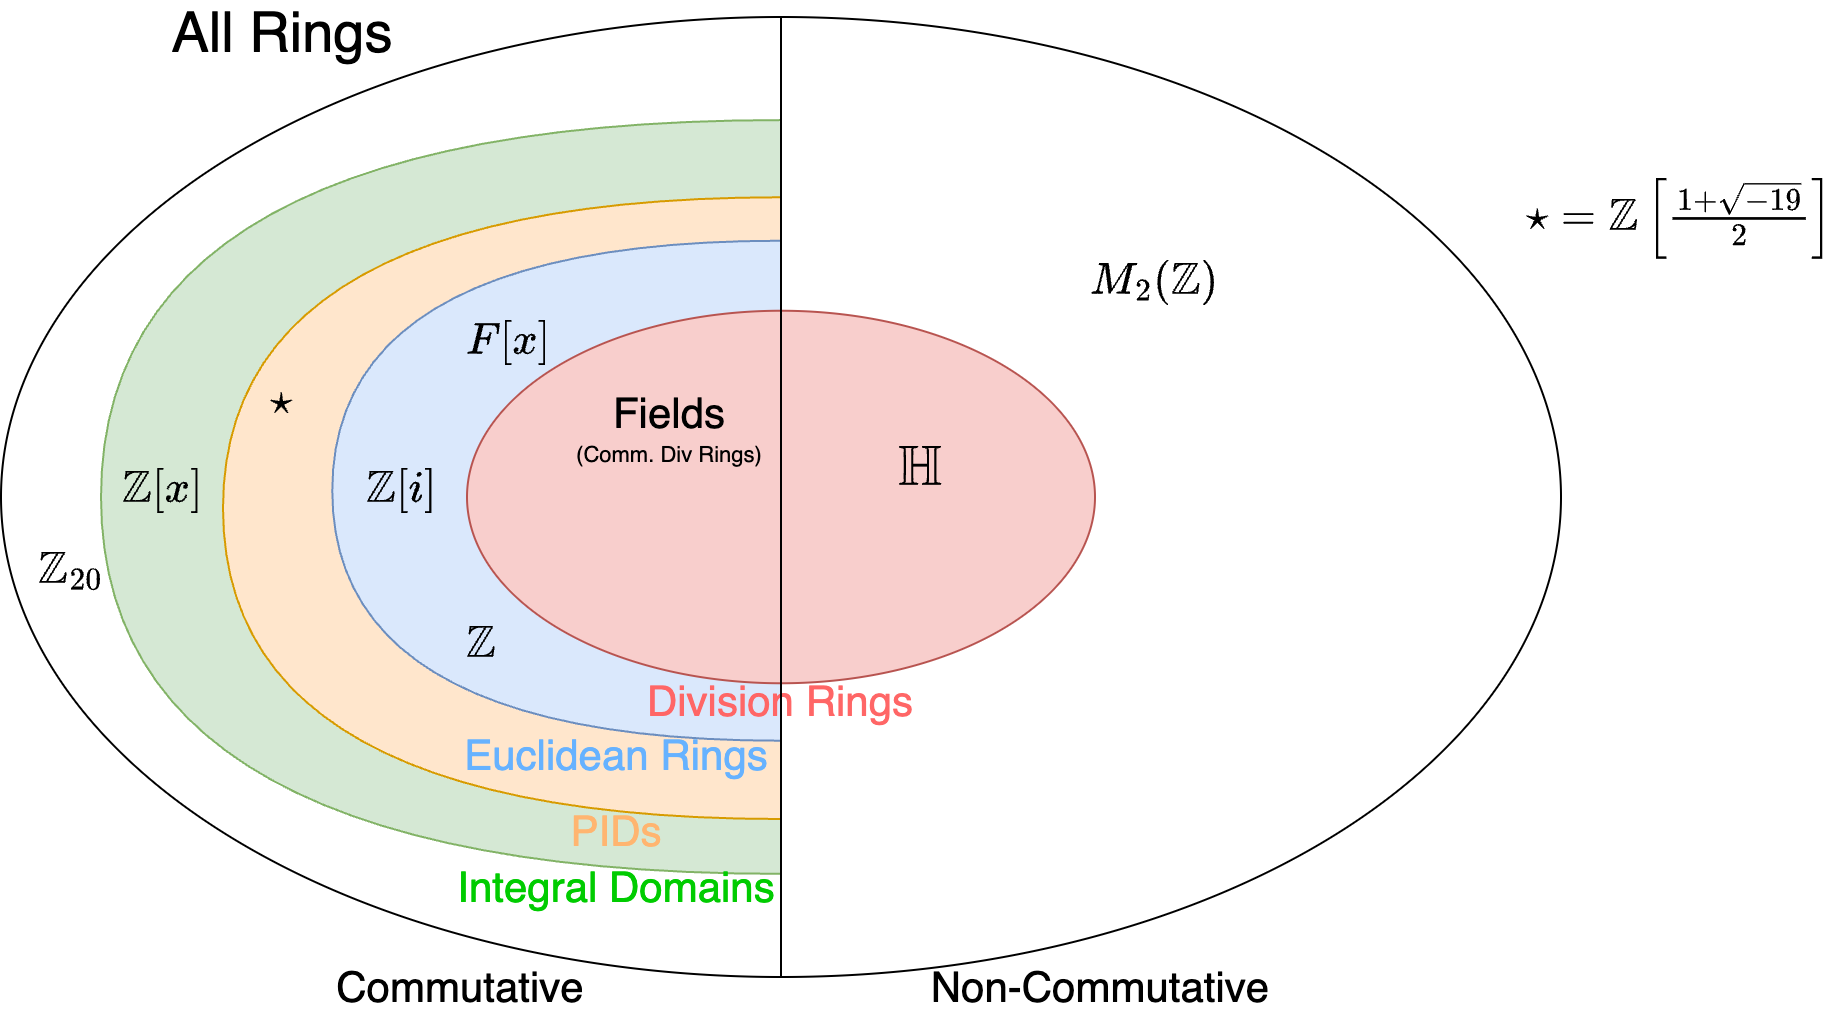
\includegraphics[width=\textwidth]{Figures/Ring Classifications_PID_not_Euc.png}
        \caption{Ring Classifications, The (mostly) complete picture}
\end{center}
\end{figure}

We end our discussion on Rings by pointing out some nuances to the classification of rings. We showed already that 
\begin{align*}
    R \text{ Euclidean} \implies \ \ R \text{ PID (every ideal has the form $Rx$ for some generator $x$)}
\end{align*}
but the converse is not true in general (i.e. $R \text{ PID }\not \implies R \text{ Euclidean}$), we will touch on an example momentarily. \\ 

But first, we would like to give an example of an integral domain that is not a PID: \\
$\Z[x]=\{\text{ polynomials with integer coefficients }\}$ is an integral domain because $\Z$ but as we will soon see it is not PID. \\
Recall: $Ra+Rb$ is an ideal called ``ideal generated by $a$ and $b$''. \\
In $\Z[x]$ consider the ideal $U$ generated by $2$ and $x$
\begin{align*}
    U=\{r(x)\cdot 2 + s(x)\cdot x \ | \ r(x), \ s(x)\in \Z[x]\}
\end{align*}
All elements in $U$ have even constant terms, so $U\varsubsetneq \Z[x]$. We will now show $\Z[x]$ contains a non-principal ideal via a contradiction:
\textit{Proof: } Assume $U$ is principal with generator $q(x)$
\begin{align*}
    U=\Z[x]q(x)
\end{align*}
Now, 
\begin{align*}
    2\in U \ \implies \ \exists \ f(x) \in \Z[x] \ni \ \ 2=\overset{\substack{\text{ non-zero so } \\ \text{both have degree} \\ \downarrow \ \ \ \ \ \ \  \downarrow \ \ \ \ }}{f(x) \cdot q(x)}
\end{align*}
Compare degrees
\begin{align*}
    0 &= \underbrace{\deg(f(x))}_{\geq 0}+\underbrace{\deg(g(x))}_{\geq 0} \\
    &\implies \deg(f(x))=\deg(g(x))=0 \\
    &\implies f(x) \text{ and }g(x) \text{ are integers, so } \underset{\substack{\uparrow \\ \text{prime...}}}{2}=\underset{\substack{\uparrow \\ \text{so, } f(x)}}{(\pm 1)}\underset{\substack{\uparrow \\ g(x)}}{(\pm 2)}
\end{align*}
Note that $g(x)\in U$ as it will be an even constant term. \\ \steezybreak
Next we have 
\begin{align*}
    x\in U &\implies \exists \ h(x) \in \Z[x]\ni \ x=h(x)\cdot g(x) \\
    &\implies x=h(x)(\pm 2) \\
    &\implies x=(nx+m)(\pm 2) \\
    &\implies x=\pm 2nx \pm 2m \\ 
    & \therefore  \ 2m =0 \ \ \ \ (\text{polynomials equal } \implies \text{ corresponding coefficients are equal})\\
    &\implies \pm 2n =1
\end{align*}
But $2$ has no inverse in $\Z$! $\Rightarrow\Leftarrow$ \\ 
$\therefore$ $U$ is not principal. \\

So $Z[x]$ contains an ideal (namely $\langle x,2 \rangle$) which is not principal, so, while it is an integral domain, it is not a PID.

Finally, without going into too much detail (see the paper if you are curious $\smiley$) we mention a PID that is not Euclidean:
\begin{align*}
    \underset{\substack{ \uparrow \\ \text{complex root} \\ \text{ of } x^2-x+5}}{\Z \left[ \frac{1+\sqrt{-19}}{2} \right] } = \left\{ a+b \left( \frac{1+\sqrt{-19}}{2} \right) \ | \ a,b \in \Z \right\}
\end{align*}
For a complete description see \href{https://www.stat.uchicago.edu/~lekheng/courses/114s09/pidnoted.pdf}{``A Principal Ideal Domain that is not a Euclidean Domain'' by Oscar A C\'{a}mpoli, American Mathematical Monthly (1988)}


\begin{tcolorbox}
    This completes the main course material for MATH 421/521. I hope you have enjoyed the material so far! \\ 
    
    Over the next few months I will begin piecing together two more chapters, one introducing Vector Spaces from this general point of view, and another which attempts to tie together, via the language of Category Theory, some of the ideas we have encountered so far. \\

    But first, I am going to work through all of the material written up to this point to try to clean up the language and formatting a bit. \\

    More fun math stuff to come, thank you for reading with me $\smiley$
\end{tcolorbox}
%\steezybreak \textit{This material onward is incomplete, more to come in the very near future!}
